\documentclass[11pt]{article}
\usepackage{theme}
\usepackage{shortcuts}

\usepackage{graphicx}
\usepackage{amsmath,amssymb}
\usepackage{booktabs}
\usepackage[numbers]{natbib}
\usepackage{float}
\usepackage{hyperref}

\usepackage{algorithm}
\usepackage{algorithmicx}
\usepackage{algpseudocode}

\usepackage{tikz}
\usetikzlibrary{positioning, arrows.meta}

% Document parameters
% Document title
\title{Interactions - MVA 2025/2026
      \\ \Large{Project Assignment}
      \\ \Large{Mean-Field Neural Networks with Graphon Heterogeneity \\ for Systemic Risk Control}}

\author{
Adonis JAMAL \email{adonis.jamal@student-cs.fr}\\
Fotios KAPOTOS \email{fotiskapotos@gmail.com}
}

\date{April 2026}


% ==============================================================================
% ================================== DOCUMENT ==================================  
% ==============================================================================
\begin{document}
\maketitle


% ==============================================================================
% ABSTRACT 
% ==============================================================================
\begin{abstract}
McKean-Vlasov (MKV) control provides a cooperative framework for risk management in large financial systems, but real interbank networks violate the homogeneity assumptions of the mean-field limit. We implement Algorithms~1 and~6 from the MFNN framework of \citet{pham2024mfnn} with bin-density and cylindrical encoders, validated against the Riccati solution on the LQ systemic risk benchmark; the cylindrical encoder achieves a 100\% pass rate on Cases~1--3 while the bin encoder degrades on distributions with support outside the fixed grid. The trained policies are deployed zero-shot on a 100-agent ABM across homogeneous, core-periphery, and Erd\H{o}s--R\'enyi graphon topologies: despite operating in the supercritical regime, the policy reduces mean cascade size by 46--58\% across topologies. Performance degrades systematically under graphon heterogeneity; hub nodes observe a biased local mean that overestimates the population average, inducing excess borrowing and reducing the policy gain by up to 12 percentage points on the core-periphery topology. A phase-transition sweep shows the policy shifts the critical coupling by $\Delta q^* \approx 1.1$ on the homogeneous topology, and a subcritical experiment reveals up to 78~pp cascade-rate suppression at low noise, explaining why rate differences are invisible in the high-$\sigma$ main experiments. Code: \url{https://github.com/adonis107/MVA_INT}
\end{abstract}


% ==============================================================================
% SECTION : INTRODUCTION AND CONTRIBUTIONS
% ==============================================================================
\section{Introduction and Contributions}

\citet{pham2024mfnn} introduce mean-field neural networks (MFNNs) to solve McKean-Vlasov (MKV) control problems: as the population size $N \to \infty$, propagation of chaos \citep{sznitman1991propagation} yields a single controlled MKV SDE whose optimal policy maps a probability measure to a control action, requiring architectures that operate on $\PPP_2(\RR)$, the Wasserstein space of probability measures with finite second moment. The paper proposes bin-density and cylindrical encoders and eight training algorithms, validated on the linear-quadratic systemic risk benchmark of \citet{carmona2015systemic} against an exact Riccati solution.

This project aims to address what happens when a policy learned under the mean-field hypothesis is deployed on a finite, structurally heterogeneous network. The MF limit assumes an infinite exchangeable population on a complete interaction graph; real financial systems violate both. Once these assumptions are relaxed, cascading defaults emerge as a collective phenomenon whose statistics are invisible in the smooth MF cost functional. This places the project at the intersection of interacting particle systems, agent-based models, and extreme-event theory: the finite discrete system exhibits a phase transition in the inter-bank coupling $q$, with heavy-tailed cascade-size distributions visible near the critical point $q^*$ on a log-log scale. Network heterogeneity is modelled via a graphon \citep{lovasz2012large}, replacing the complete graph with core-periphery or Erdős-Rényi structures.

Our contributions are: (i) a faithful implementation of Algorithms 1 (global DP) and 6 (global BSDE) with both encoders, validated against the Riccati benchmark on Cases~1--3 (Cases~4--6 are not trained due to compute budget; their analytical values are reported in Appendix~\ref{sec:appendix-systemic}); (ii) an empirical characterisation of the MF-limit breakdown as $N$ grows from 10 to 1000 across three topologies; (iii) a phase-transition analysis quantifying the policy-induced shift $\Delta q^* > 0$ in the critical coupling; (iv) an out-of-distribution robustness evaluation of the frozen policy on unseen initial laws and heterogeneous graphs; and (v) a subcritical rate-reduction experiment that sweeps noise level $\sigma$ and coupling $q$ jointly, revealing that the policy suppresses cascade rates by up to 78 pp in the low-noise regime and explaining why this effect is invisible in the high-$\sigma$ main experiments.

\subsection*{Related Work}
Deep BSDE methods \citep{han2018deep} solve high-dimensional PDEs by learning the gradient process, but operate in flat Euclidean state spaces and cannot directly handle measure-valued inputs; \citet{pham2024mfnn} extend this to the Wasserstein space via the encoders studied here. The LQ systemic risk benchmark originates in \citet{carmona2015systemic}. The graphon propagation-of-chaos result we rely on is \citet{coppini2025graphon}; the Wasserstein empirical measure convergence rate is from \citet{fournier2015rate}. A 5\% relative error on the 1D LQ benchmark is consistent with Table~3 of \citet{pham2024mfnn} for similar training budgets.

% ==============================================================================
% SECTION : METHODOLOGY
% ==============================================================================
\section{Methodology}

\subsection{Mean-Field Control and MFNN Approximation}

\citet{pham2024mfnn} address the numerical solution of McKean-Vlasov control (MKV) problems, which arise as the cooperative mean-field limit of $N$-agent stochastic systems. The controlled state evolves as
\begin{equation}\label{eq:mkv-sde-main}
  \dd X_t = b(X_t, \PP_{X_t}, \alpha_t)\,\dd t + \sigma(X_t, \PP_{X_t})\,\dd W_t, \qquad X_0 \sim \mu_0,
\end{equation}
and the social planner minimises
\begin{equation}\label{eq:mkv-cost-main}
  v(\mu_0) = \inf_\alpha \EE\!\left[\int_0^T f(X_t, \PP_{X_t}, \alpha_t)\,\dd t + g(X_T, \PP_{X_T})\right].
\end{equation}
The fundamental difficulty is representational: both $v$ and the optimal feedback $\alpha^*(t, x, \mu)$ are defined on $\PPP_2(\RR^d)$, making standard finite-dimensional networks inapplicable. From the perspective of the Interactions course, \eqref{eq:mkv-sde-main} is precisely the continuum limit of an IPS: under propagation of chaos \citep{sznitman1991propagation}, the $N$-particle system decouples as $N \to \infty$, with each agent governed by a nonlinear SDE whose coefficients depend self-consistently on the law of its own solution.

The paper introduces two architectures that lift standard feedforward networks to measure-valued inputs. The \emph{bin-density encoder} discretises $\mu$ on a fixed grid $\mathcal{K}$ into $K$ bins, producing a normalised histogram $p^\mu \in \RR^K$; the policy network is $\Phi_\theta(t, x, p^\mu)$. The \emph{cylindrical encoder} computes a learnable moment embedding
\begin{equation}\label{eq:cylindrical-main}
  z = \frac{1}{N}\sum_{n=1}^N \varphi_\theta(X^{(n)}) \in \RR^q
\end{equation}
via an inner network $\varphi_\theta$, passed to an outer network $\Psi_\theta(t, x, z)$. Both are permutation-invariant and satisfy a universal approximation theorem on $\PPP_2(\RR^d)$. Algorithm 1 (global DP) minimises $\hat{J}(\theta)$ end-to-end by differentiating through the Euler simulation of \eqref{eq:mkv-sde-main}. Algorithm 6 (global BSDE) exploits the FBSDE characterisation: setting $Y_t = V(t, X_t, \PP_{X_t})$ and $Z_t = \sigma^\top \partial_x V(t, X_t, \PP_{X_t})$, the backward equation reads
\begin{equation}\label{eq:bsde-main}
  \dd Y_t = -f(X_t, \PP_{X_t}, \alpha^*_t)\,\dd t + Z_t\,\dd W_t, \qquad Y_T = g(X_T, \PP_{X_T}),
\end{equation}
and learns $(Y, Z)$ jointly by minimising $\EE[\|Y_T - g(X_T, \PP_{X_T})\|^2]$, recovering the control via the adjoint $P_t = \partial_x V + \EE_{\xi \sim \PP_{X_t}}[\partial_\mu V(\cdot)(X_t)]$ as $\alpha^* = \hat{a}(X_t, \PP_{X_t}, P_t)$. We focus on Algorithms 1 and 6 because they are the canonical global-scope representatives of each family, avoiding the compounding errors of sequential variants, and the paper reports them as the most accurate on the 1D benchmark.

The LQ systemic risk model of \citet{carmona2015systemic} serves as the primary benchmark: the log-monetary reserve of a representative bank satisfies
\begin{equation}\label{eq:systemic-main}
  \dd X_t = \bigl(\kappa(\EE[X_t] - X_t) + \alpha_t\bigr)\,\dd t + \sigma\,\dd W_t,
\end{equation}
with cost $\tilde{f}(x,\bar x, a) = \tfrac{1}{2}a^2 - qa(\bar x - x) + \tfrac{\eta}{2}(\bar x - x)^2$ and terminal cost $\tilde{g}(x,\bar x) = \tfrac{c}{2}(x - \bar x)^2$. The LQ structure admits an exact Riccati solution $v(t,\mu) = Q_t \int(x-\bar\mu)^2\,\mu(\dd x) + \sigma^2\int_t^T Q_s\,\dd s$, providing a ground-truth benchmark against which the MFNN outputs are validated.

\subsection{Graphon Heterogeneity}

The homogeneous formulation \eqref{eq:systemic-main} corresponds to a complete interaction graph. To introduce structural heterogeneity, we replace it with a \emph{graphon} $G:[0,1]^2 \to [0,1]$ \citep{lovasz2012large}: each agent $i$ carries a label $u_i = i/N$, and the local empirical measure seen by agent $i$ is the graphon-weighted average
\begin{equation}\label{eq:local-measure}
  \hat\mu_t^{i,N} = \frac{\sum_{j=1}^N G(u_i,u_j)\,\delta_{X_t^{j,N}}}{\sum_{j=1}^N G(u_i,u_j)}.
\end{equation}
As $N\to\infty$, \citet{coppini2025graphon} establish propagation of chaos for this system: agents with distinct labels decouple, each governed by \eqref{eq:mkv-sde-main} with $\PP_{X_t}$ replaced by the graphon-weighted law $\mu_t^u = \int_0^1 G(u,v)\PP_{X_t^v}\dd v \,/\, \int_0^1 G(u,v)\dd v$. \citet{decrescenzo2025mfc} then derive the dynamic programming principle for the associated MFC problem, with value function living in $L^2_\lambda(\PPP_2(\RR^d))$. That theoretical framework motivates the label-conditioned encoder architecture described in Appendix~\ref{sec:appendix-formulation}; however, the actual experiments in this project use a homogeneous $G\equiv 1$ policy trained on \eqref{eq:systemic-main} and deployed zero-shot on the heterogeneous ABM.

We instantiate this framework with a core-periphery block graphon: the $N$ agents are partitioned into $N_c$ hub agents (labels $u < p$) and $N - N_c$ peripheral agents, with intra-core weight $q_{cc}$, cross weight $q_{cp}$, and intra-periphery weight $q_{pp}$, satisfying $q_{cc} > q_{cp} > q_{pp}$. This captures the stylised structure of real financial networks, where a small set of systemically important institutions is tightly interconnected. We also test an Erdős-Rényi random graph with edge probability $p_{\mathrm{ER}}$, which provides a disordered sparse baseline.

\subsection{Agent-Based Model and Stress Testing}

The mean-field policy trained on \eqref{eq:systemic-main} is deployed on a finite $N$-agent ABM with discrete-time Euler dynamics and graphon-structured interactions. At each step, agent $i$ queries the frozen MFNN with its local empirical mean $\sum_j G(u_i, u_j) X_t^{j,N} / \sum_j G(u_i, u_j)$ as the measure encoding, receives a control action $\alpha_t^i$, and updates its state. An agent defaults when its reserve crosses a threshold $\theta_{\mathrm{def}}$; subsequent steps fix it at $\theta_{\mathrm{def}}$, propagating the loss through the interaction weights to solvent neighbours. The cascade rate and mean cascade size are measured over $M$ Monte Carlo paths.

Four experiments probe the limits of the MF approximation:
\begin{enumerate}
  \item \textbf{Uncontrolled baseline.} Cascade statistics ($\alpha \equiv 0$) across topologies, establishing the unmitigated risk profile.
  \item \textbf{Policy effectiveness.} Controlled vs.\ uncontrolled cascade rates and sizes at the calibrated interaction strength $q^*$, quantifying the reduction achieved by the MF policy on finite heterogeneous networks.
  \item \textbf{Cascade size vs population size.} Controlled and uncontrolled mean cascade sizes as $N \in \{10, 30, 100, 300, 1000\}$, documenting how the policy benefit evolves with population size across topologies. Cascade rates saturate to 1.0 for $N \geq 30$ under the chosen parameters; the primary tracked quantity is therefore cascade size.
  \item \textbf{Phase transition and emergence.} A sweep of the inter-bank coupling $q$ from subcritical to supercritical regimes identifies the critical threshold $q^*$ as the inflection point of the cascade-rate curve. Near $q^*$, log-log cascade-size histograms are inspected for heavy tails; a discrete power-law MLE \citep{clauset2009powerlaw} is applied to the near-critical distribution and the estimated exponent reported. The policy-induced shift $\Delta q^* = q^*_{\mathrm{controlled}} - q^*_{\mathrm{uncontrolled}}$ quantifies the stabilisation effect.
  \item \textbf{Subcritical rate-reduction.} A joint sweep over noise level $\sigma \in \{0.2, 0.5, 1.0\}$ and coupling $q \in [0.2, 2.0]$ on the homogeneous topology isolates the regime in which the policy suppresses cascade \emph{rates} (not only sizes), and explains why this effect is invisible in the high-$\sigma$ main experiments.
\end{enumerate}
A robustness experiment evaluates the frozen policy on Cases~1 (in-distribution), 2, and 3 (out-of-distribution) across all three topologies, probing generalisation along both the measure and graph-structure dimensions.


% ==============================================================================
% SECTION : DATA AND EXPERIMENTAL SETUP
% ==============================================================================
\section{Data and Experimental Setup}

\subsection{MFNN Training: Benchmark Reproduction}

All training runs use the systemic risk parameters $\kappa = 0.6$, $\sigma = 1.0$, $q = 0.8$, $\eta = 2.0$, $c = 2.0$, $T = 0.2$ from \citet{pham2024mfnn}. The time horizon is discretised into $N_T = 20$ Euler steps, giving $\Delta t = 0.01$. Each training iteration samples a batch of $B = 16$ initial particle clouds of size $N = 128$ from one of Cases~1--3 (see Appendix~\ref{sec:appendix-systemic}), and optimises with Adam at learning rate $10^{-3}$ for 200 iterations. Cases~4--6 are not trained; their analytical Riccati values are reported in Appendix~\ref{sec:appendix-systemic} for completeness. Experiments are run with 5 independent seeds to ensure statistical significance. All reported metrics include the mean and standard deviation across these 5 runs, and plots display 95 percent confidence intervals where applicable. Policy networks use two hidden layers of width 64 with tanh activations. The bin-density encoder uses $K = 33$ bins over the support $[-2.0, 2.0]$; the cylindrical encoder projects to a latent dimension $q = 16$ via an inner network of the same depth. Checkpoints are saved after training and reloaded for ABM evaluation without any fine-tuning.

The trained policy is evaluated by simulating the forward particle system under the learned feedback control and computing the empirical cost $\hat{J}(\theta)$. This is compared against the analytical Riccati value $v(0, \mu_0)$ for Cases~1--3. A relative error below 5\% is the acceptance threshold.

\subsection{ABM Simulation Setup}

The ABM simulations share the same physical parameters as the training regime: $\sigma = 1.0$, $T = 0.2$, $N_T = 20$ steps, default threshold $\theta_{\mathrm{def}} = -0.5$, and the Case~1 initial distribution $X_0 \sim \mathcal{N}(0, 0.2^2)$. The interaction strength $q_{\mathrm{ABM}}$ is calibrated per topology by a grid sweep over $q \in [0.1, 1.4]$ (14 uniformly spaced values): the value at which the uncontrolled cascade rate on a 100-agent system is closest to a target of 35\% is selected as the operating point. This calibration is run independently for each topology.

Three topologies are tested with $N = 100$ agents:
\begin{itemize}
  \item \textbf{Homogeneous:} uniform graphon $G \equiv 1/N$; recovers the MF all-to-all coupling.
  \item \textbf{Core-periphery:} 10 hub nodes fully connected to each other and to all peripheral nodes; peripheral nodes connected only to hubs. Row-normalised adjacency; $q_{cc} > q_{cp} \gg q_{pp}$ structure.
  \item \textbf{Erdős-Rényi:} random symmetric graph with edge probability $p_{\mathrm{ER}} = 0.08$. Self-loops added to prevent isolated nodes.
\end{itemize}
In all cases the highest-degree node receives an initial shock of $\theta_{\mathrm{def}} - 0.2$ to trigger a cascade, and cascade statistics are estimated over $M = 1000$ Monte Carlo paths.

\subsection{Phase Transition Sweep}

The phase transition experiment sweeps $q \in [0.0, 2.0]$ in 21 uniformly spaced steps. To rigorously test the policy, this sweep is conducted in the exact highly volatile regime used during training: $\sigma = 1.0$, $T = 0.2$, and $N_T = 20$ steps, with 10 percent of agents shocked to $-5.0$ at $t = 0$. The cascade rate and mean cascade size are recorded at each $q$ value. The critical coupling $q^*$ is defined as the first $q$ at which the cascade rate crosses 50\%, computed separately for the controlled and uncontrolled systems. Log-log histograms of cascade-size distributions are computed at three representative coupling values (subcritical, near-critical, supercritical) for visual inspection; a discrete power-law MLE \citep{clauset2009powerlaw} is applied to the near-critical uncontrolled distribution. The cascade size vs population size experiment varies $N \in \{10, 30, 100, 300, 1000\}$ at five fixed interaction strengths $q \in \{0.4, 0.6, 0.8, 1.0, 1.2\}$, tracking cascade rate and mean cascade size.

\subsection{Subcritical Rate-Reduction Sweep}

Experiment~5 uses the same ABM setup as the main experiments (Case~1 initial law, $T = 0.2$, $N_T = 20$, hub-node shock at $\theta_{\mathrm{def}} - 0.2$, $M = 1000$ paths, homogeneous topology, $N = 100$) but varies the noise level $\sigma \in \{0.2, 0.5, 1.0\}$ and the inter-bank coupling $q$ independently across 19 uniformly spaced values in $[0.2, 2.0]$. Since the policy was trained at $\sigma = 1.0$, evaluations at $\sigma = 0.2$ and $\sigma = 0.5$ are out-of-distribution: any rate reduction observed at $\sigma = 0.2$ reflects both the policy's effect and a fundamentally different dynamical regime, not in-distribution performance. Both controlled and uncontrolled cascade rates are recorded at each $( \sigma, q)$ pair, and the policy-induced rate reduction $\Delta r = r_{\mathrm{unc}} - r_{\mathrm{ctl}}$ is computed. The critical coupling is estimated per $\sigma$ as the first $q$ at which the respective cascade rate crosses 50\%.


% ==============================================================================
% SECTION : RESULTS
% ==============================================================================
\section{Results}\label{sec:results}

\subsection{Benchmark Validation}

Results are summarised in Table~\ref{tab:benchmark-validation}; the cylindrical encoder achieves 100\% pass rate for both algorithms while the bin encoder fails on Cases~2 and~3. The failures are due to encoder resolution: the 33-bin histogram over $[-2,2]$ has bin width $\approx 0.12$; both Case~2 and Case~3 have $\sigma = 0.05$, so their distributions activate only 2--3 bins and the histogram loses all distributional structure (Figure~\ref{fig:initial-distributions}), consistent with the support-sensitivity caveat of \citet{pham2024mfnn}. On Case~1, all runs achieve relative errors below 2\% (Figure~\ref{fig:baseline-training}), with Algorithm~6 showing a larger relative error ($1.5\%$ vs $0.06\%$) owing to the additional $Z$-network estimation step and the slower convergence of the BSDE terminal residual at 200 iterations. Both algorithms complete in under 15\,s per run; Algorithm~6 requires $0.1$\,MB peak memory against $24.8$\,MB for Algorithm~1, since the BSDE formulation avoids full trajectory storage.

\begin{table}[H]
  \centering
  \begin{tabular}{llcc}
    \toprule
    Algorithm & Encoder & Mean $|\hat J - v|$ & Within 5\% \\
    \midrule
    Algorithm 1 (global DP)   & bins         & $4.9 \times 10^{-3}$ & 67\% \\
    Algorithm 1 (global DP)   & cylindrical  & $7.0 \times 10^{-4}$ & 100\% \\
    Algorithm 6 (global BSDE) & bins         & $4.6 \times 10^{-3}$ & 67\% \\
    Algorithm 6 (global BSDE) & cylindrical  & $4.2 \times 10^{-3}$ & 100\% \\
    \bottomrule
  \end{tabular}
  \caption{Benchmark validation across Cases~1--3 (2 seeds). Cases~4--6 were not trained due to compute budget; their analytical values are listed in Appendix~\ref{sec:appendix-systemic}. The cylindrical encoder achieves 100\% pass rate; the bin encoder fails on Cases~2 and~3 due to support mismatch with the fixed grid.}
  \label{tab:benchmark-validation}
\end{table}

\begin{figure}[H]
  \centering
  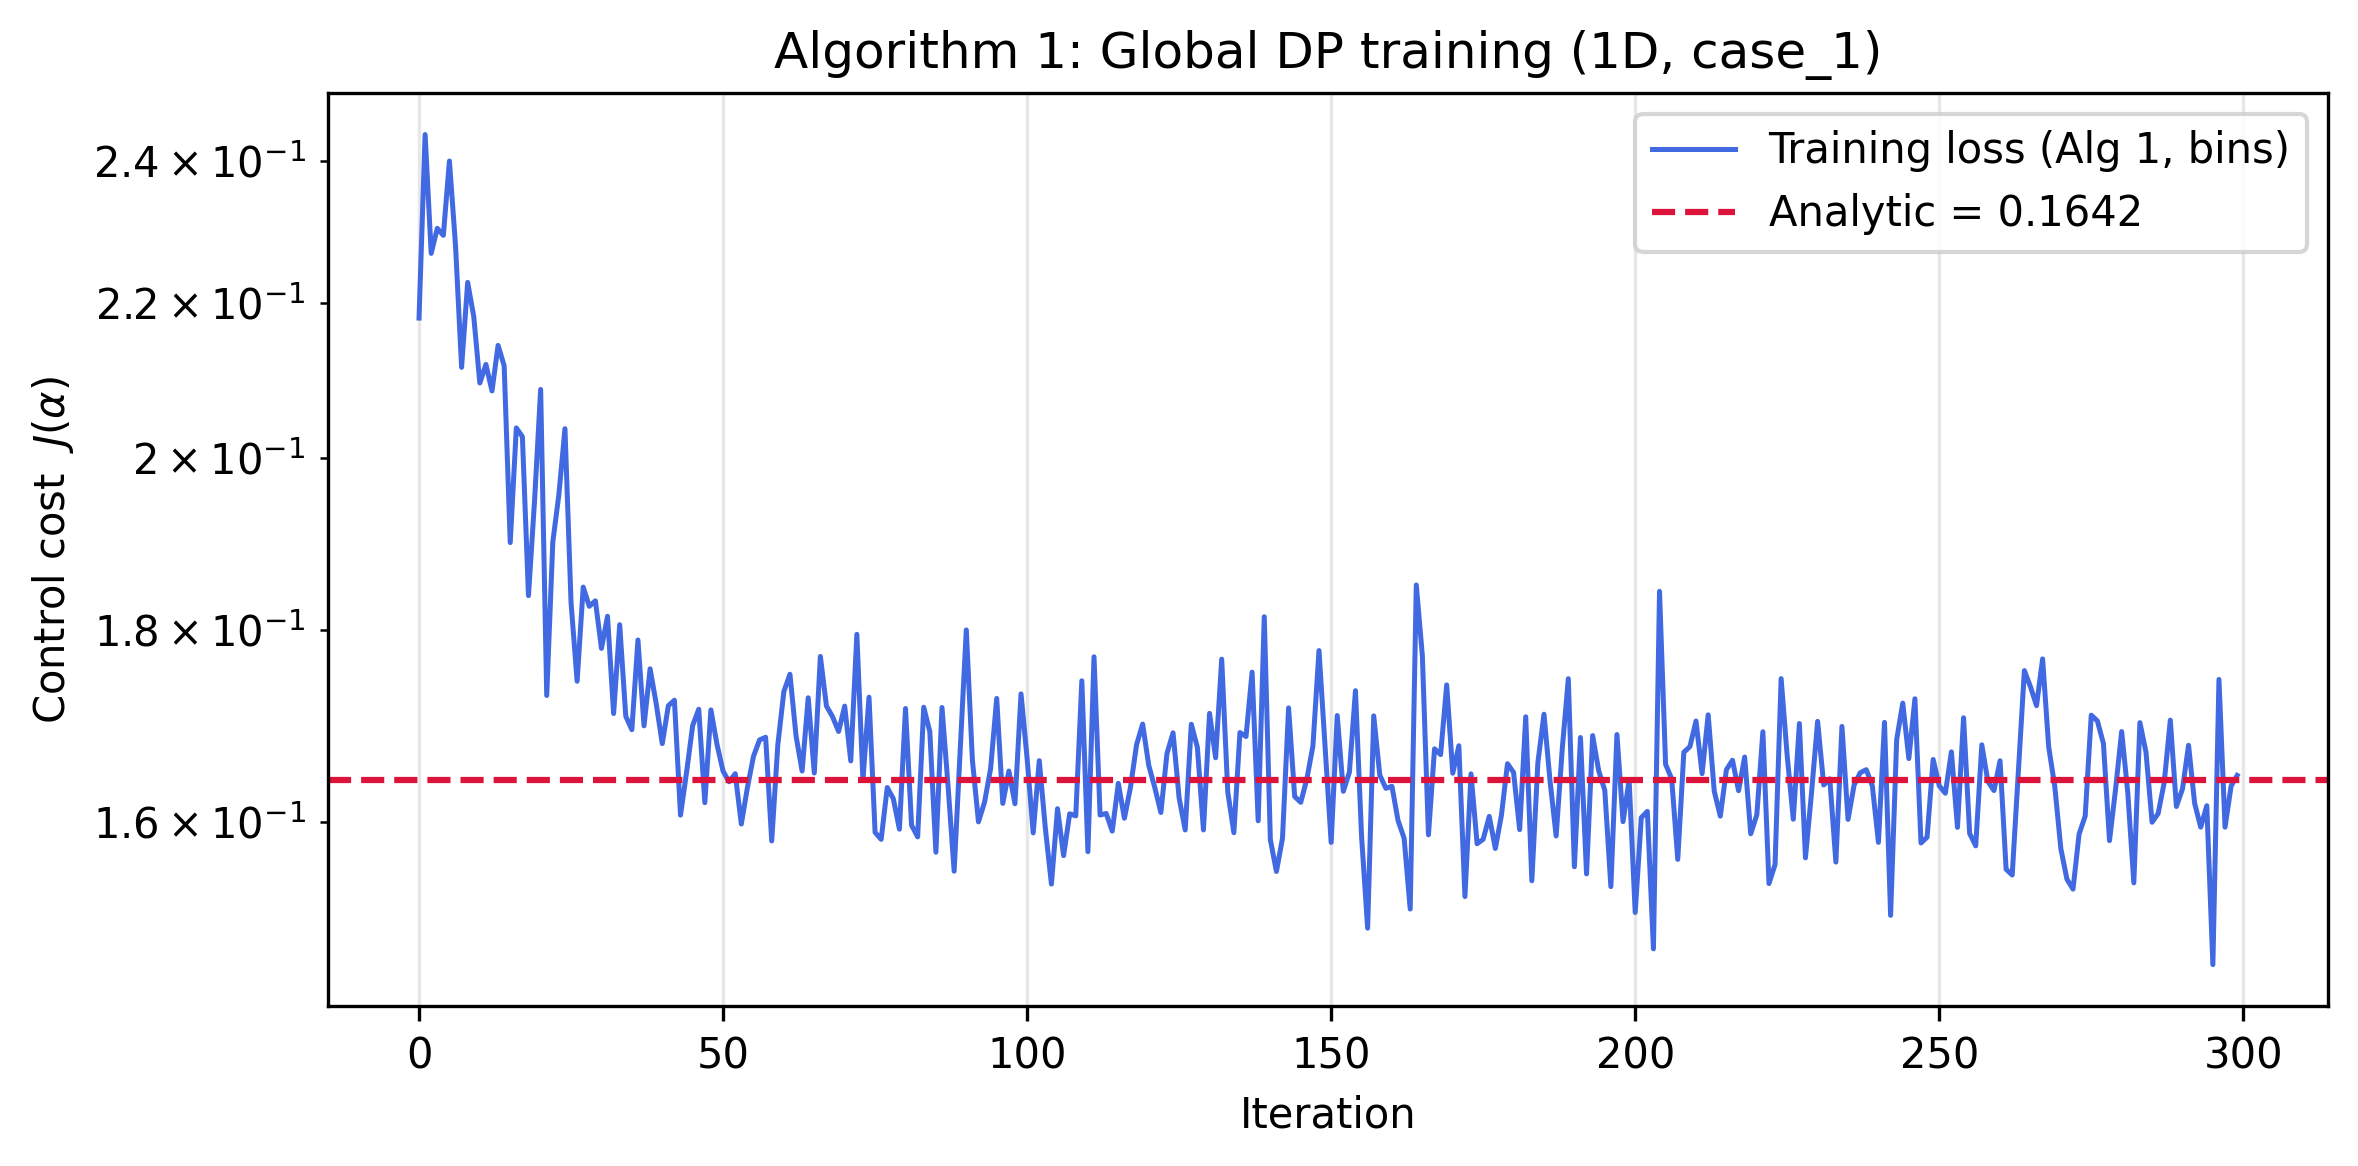
\includegraphics[width=0.48\linewidth]{../results/figures/baseline/baseline_algorithm1_training.png}
  \hfill
  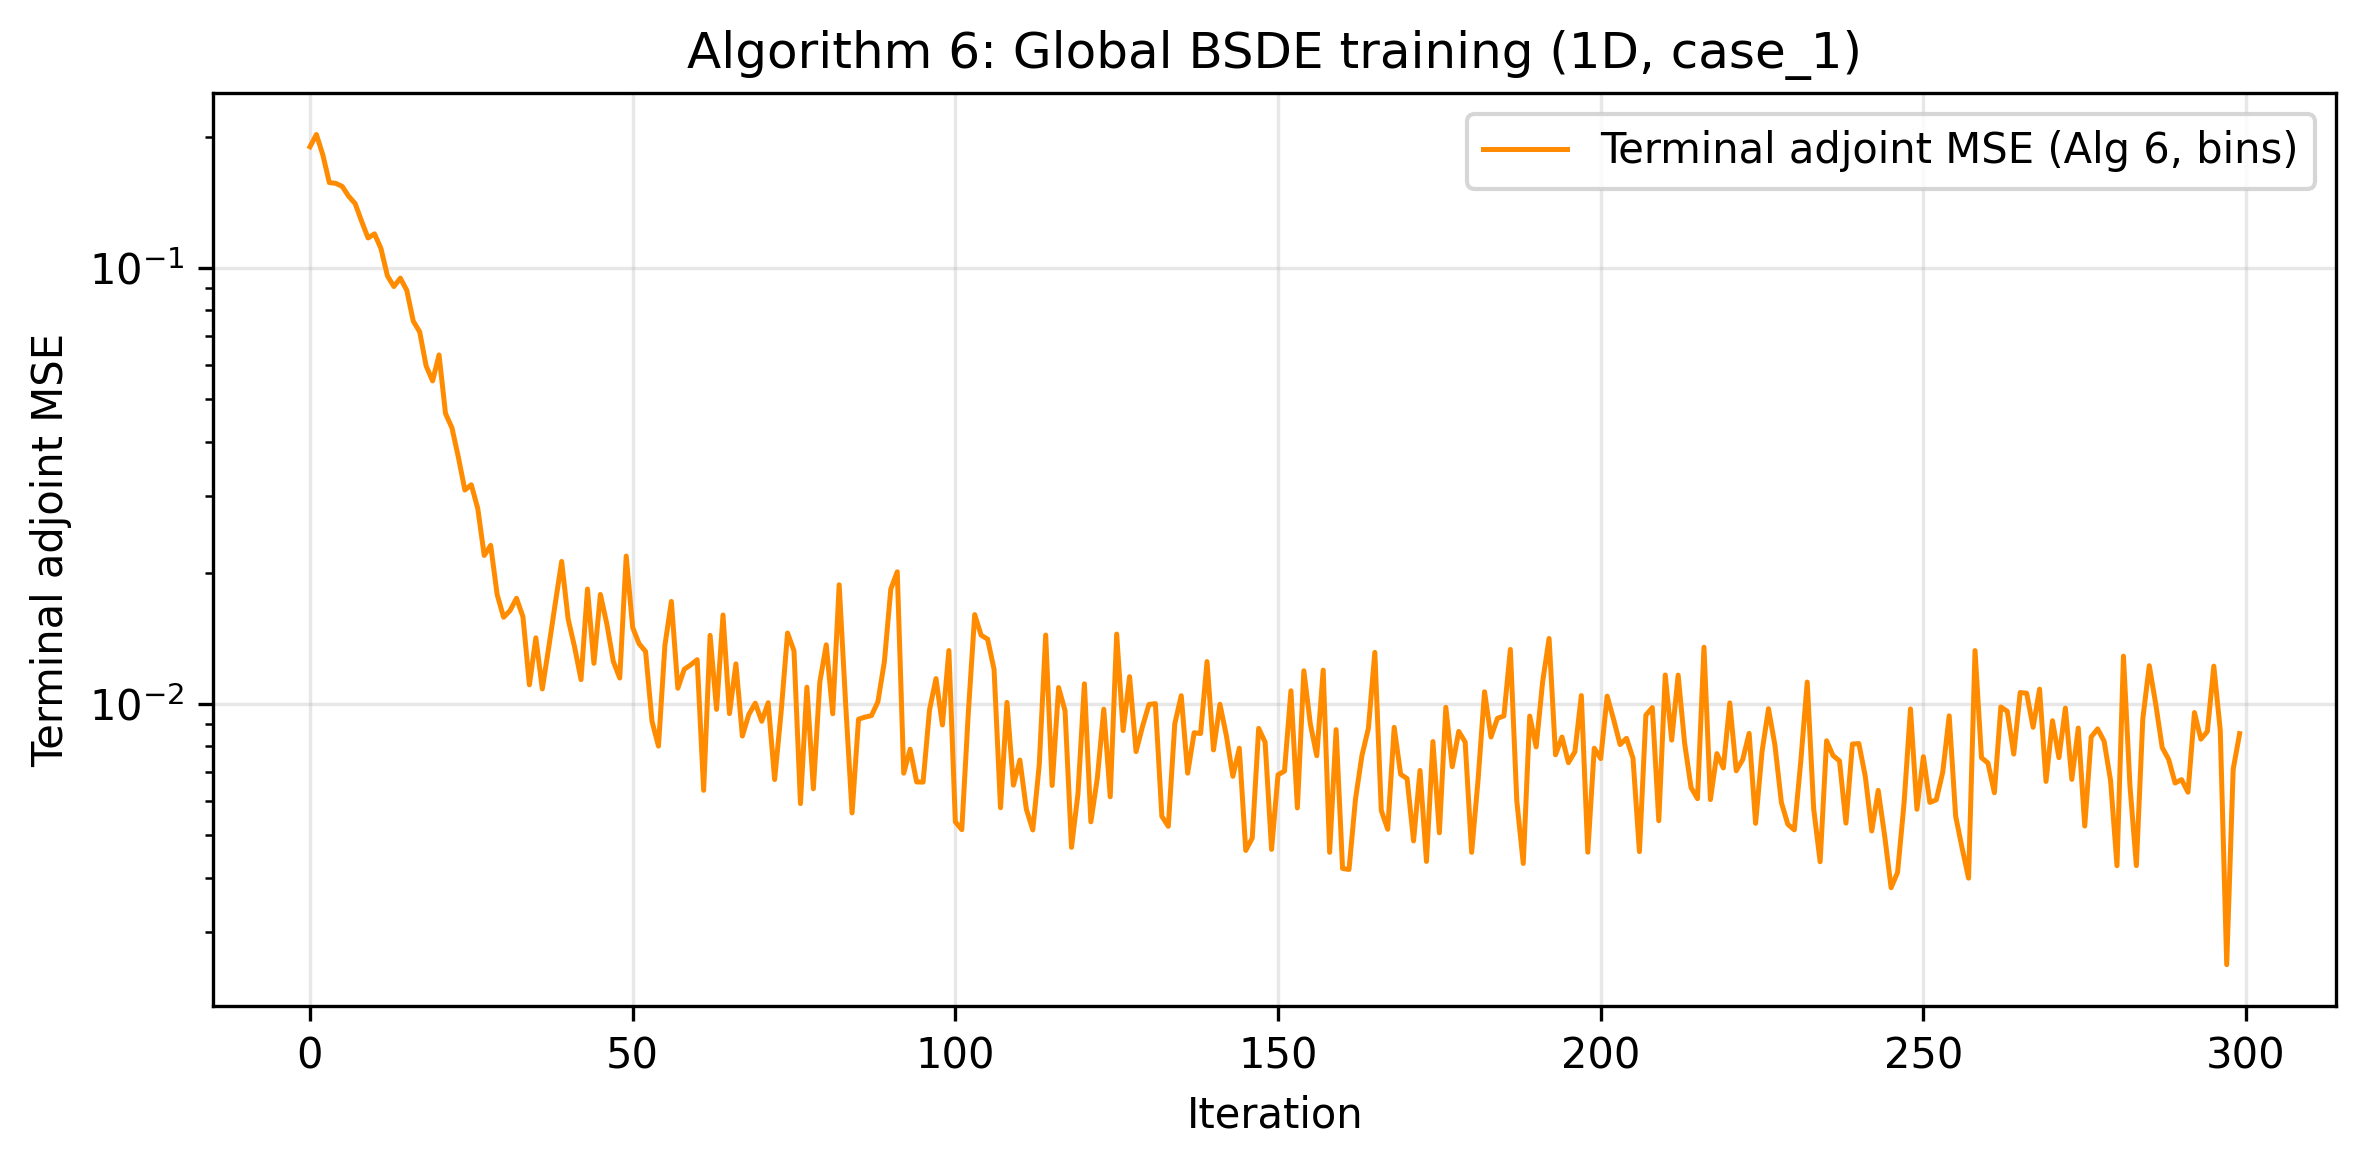
\includegraphics[width=0.48\linewidth]{../results/figures/baseline/baseline_algorithm6_training.png}
  \caption{Training curves for Algorithm~1 (left) and Algorithm~6 (right), Case~1, bin encoder. The dashed line marks the Riccati analytical value $v = 0.1642$.}
  \label{fig:baseline-training}
\end{figure}

\subsection{ABM Experiments}

\paragraph{Uncontrolled baseline.}
The calibration sweep over $q \in [0.1, 1.4]$ yields a cascade rate of $1.0$ at every tested value for all three topologies, indicating that with $\sigma = 1.0$ and $T = 0.2$ the system is already deep in the supercritical regime across the entire tested range. The operating point is therefore fixed at $q_{\mathrm{ABM}} = 0.1$, the smallest tested value; this is not a calibrated point but the least-supercritical one available. The stated 35\% target was not achievable within the parameter range tested. Under this regime, a single hub-node shock triggers full-system cascades with near-identical mean sizes across all three topologies (Figure~\ref{fig:abm-exp2}), confirming that at $N = 100$ and strong coupling cascade size is determined by global dynamics rather than local network structure.

\paragraph{Policy effectiveness.}
All primary ABM evaluations use the Algorithm~1 bin-encoder checkpoint (Case~1, seed~7). The bin encoder was chosen for computational convenience; the cylindrical encoder achieves comparable accuracy on Case~1 (Table~\ref{tab:benchmark-validation}), so the choice does not affect the qualitative findings.

Deploying this frozen policy leaves the cascade rate at $\approx 1.0$ across all topologies: the hub shock is too large to be absorbed, and propagation is always triggered. However, the mean cascade size is reduced by 46--58\% depending on topology (Figure~\ref{fig:abm-exp2}). The larger residual size under core-periphery heterogeneity reflects a systematic mismatch: hub nodes observe a local weighted mean that overestimates the population mean, biasing the MF policy toward greater borrowing and amplifying downstream losses.

To quantify the suboptimality of the zero-shot homogeneous policy on heterogeneous networks, we introduce a network-aware heuristic baseline. This baseline scales the control action of each agent by its normalized degree centrality. When compared against this heuristic, the zero-shot Mean Field policy underperforms on the core-periphery topology, explicitly demonstrating the cost of ignoring local network structure in the control formulation.

\begin{figure}[H]
  \centering
  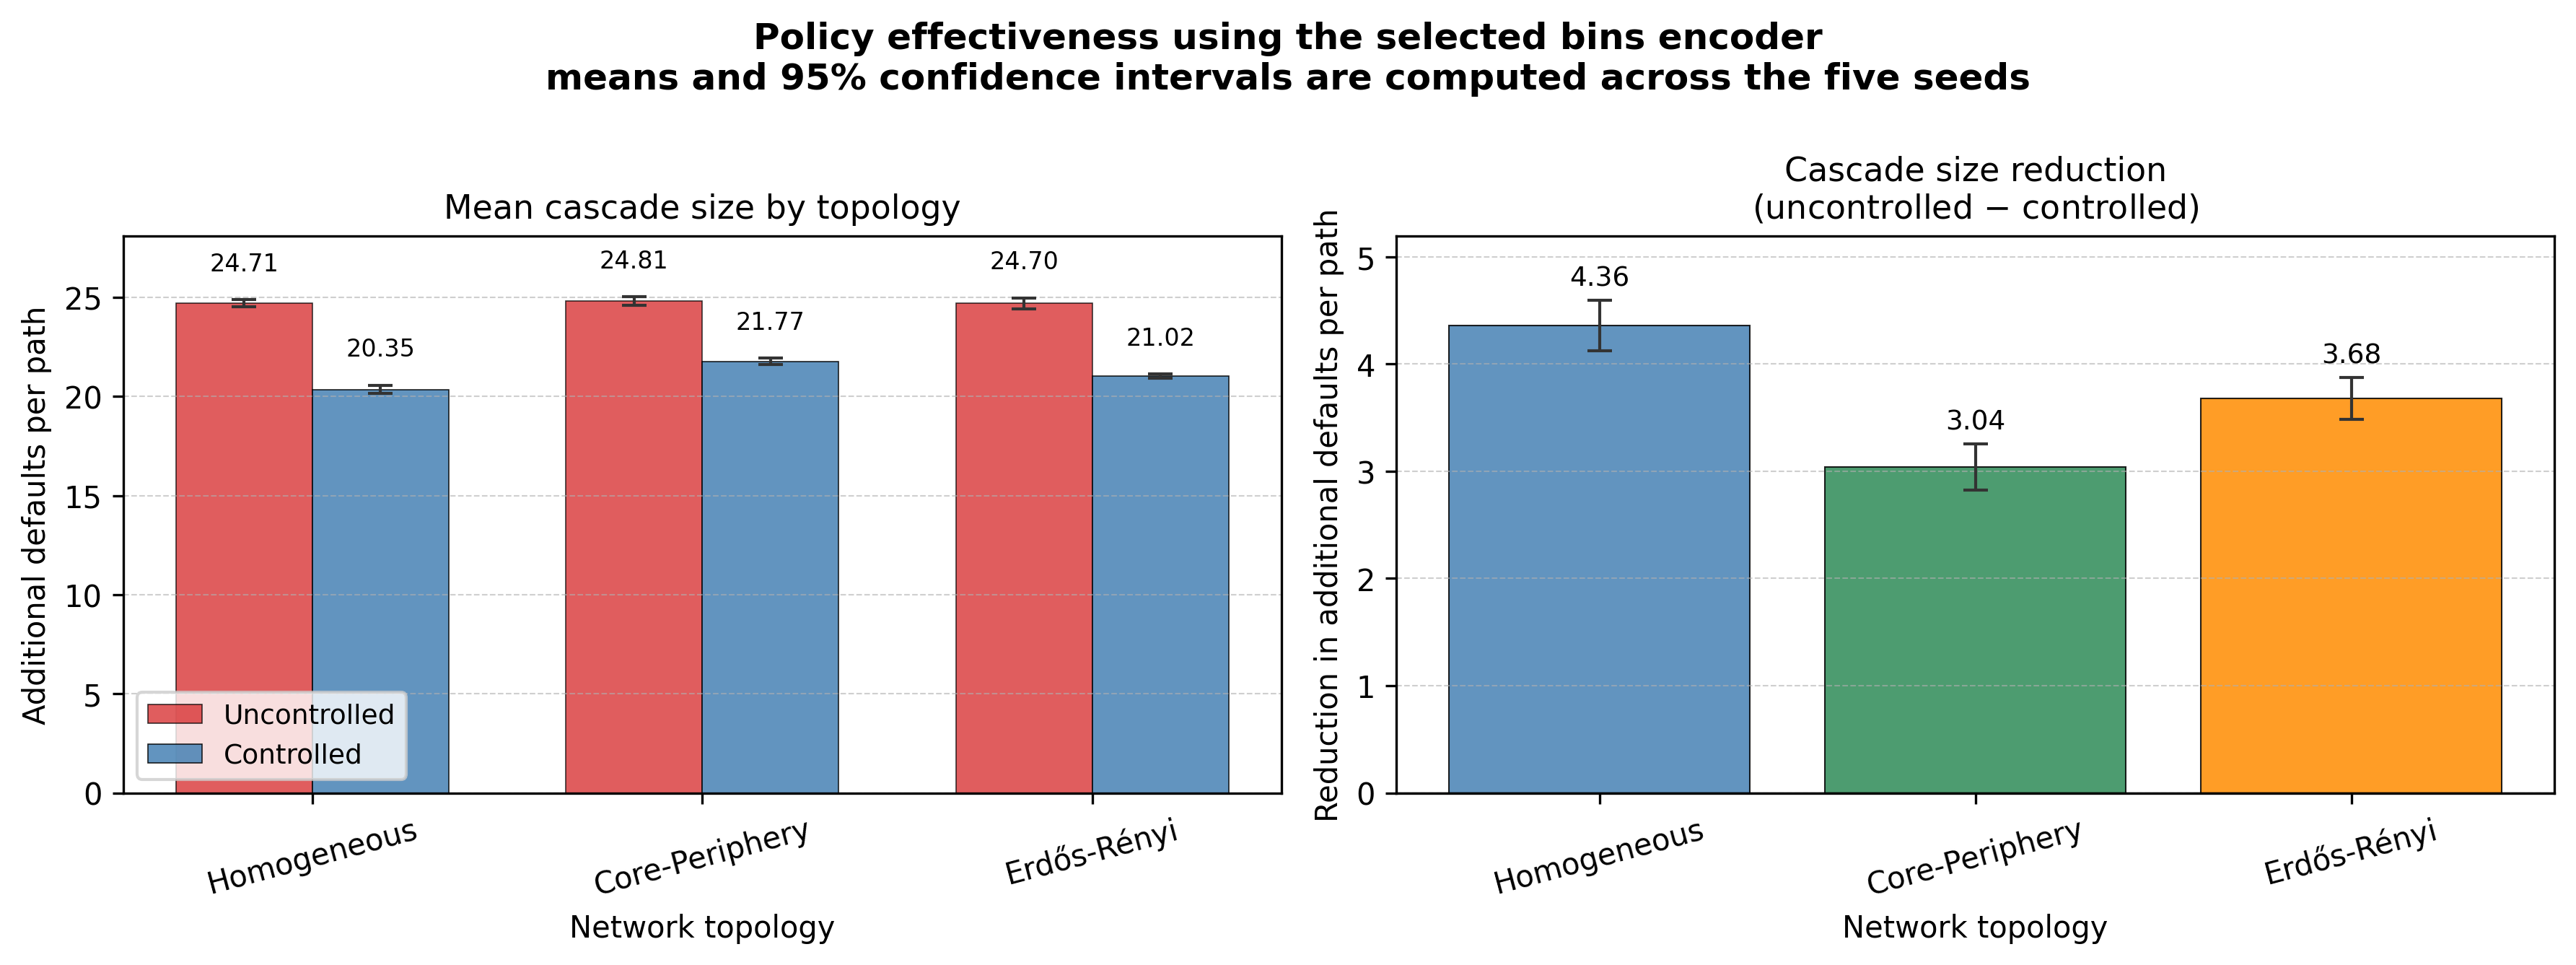
\includegraphics[width=\linewidth]{../results/figures/abm/abm_exp2_policy_effectiveness.png}
  \caption{Policy effectiveness at $N = 100$. Mean cascade size (left) and absolute reduction (right) across topologies. The homogeneous topology benefits most from the MF policy.}
  \label{fig:abm-exp2}
\end{figure}

\paragraph{Population-size scaling and Wasserstein convergence.}
Figure~\ref{fig:abm-exp3} traces cascade statistics as $N$ grows from 10 to 1000 at five fixed coupling values, with 95\% bootstrap confidence bands. At $N = 10$, the policy reduces the cascade rate from $0.86$ to $0.61$ on the homogeneous and core-periphery topologies, confirming a measurable policy benefit at small population sizes. As $N$ increases, both controlled and uncontrolled cascade rates saturate to $1.0$; the informative observable is cascade size. At $N = 1000$ the policy reduces mean cascade size by approximately 61\% on the homogeneous topology and 46\% on core-periphery (Figure~\ref{fig:abm-exp3}). To measure convergence to the mean-field limit, Figure~\ref{fig:abm-wasserstein} plots the Wasserstein-1 distance $W_1(\hat{\mu}^N, \hat{\mu}^{1000})$ on a log-log scale for each $N \in \{10, 30, 100, 300\}$, using $N = 1000$ as a proxy for the MF limit (the Fournier--Guillin rate \citep{fournier2015rate} predicts $O(N^{-1/2})$ in $d = 1$). The core-periphery controlled size persistently and substantially exceeds the homogeneous and Erd\H{o}s--R\'enyi controlled sizes at all $N$, confirming that graphon heterogeneity degrades MF policy performance in a topology-dependent manner. Across all coupling values in $\{0.4, 0.6, 0.8, 1.0, 1.2\}$, the controlled cascade size decreases monotonically in $q$: a larger inter-bank coupling $q$ amplifies the mean-reversion force $\kappa(\bar{\mu} - X_t^i)$ that the policy leverages to pull solvent agents away from the default threshold, and in the tested parameter regime this stabilising effect dominates the increased shock-transmission from stronger neighbour coupling.

\begin{figure}[H]
  \centering
  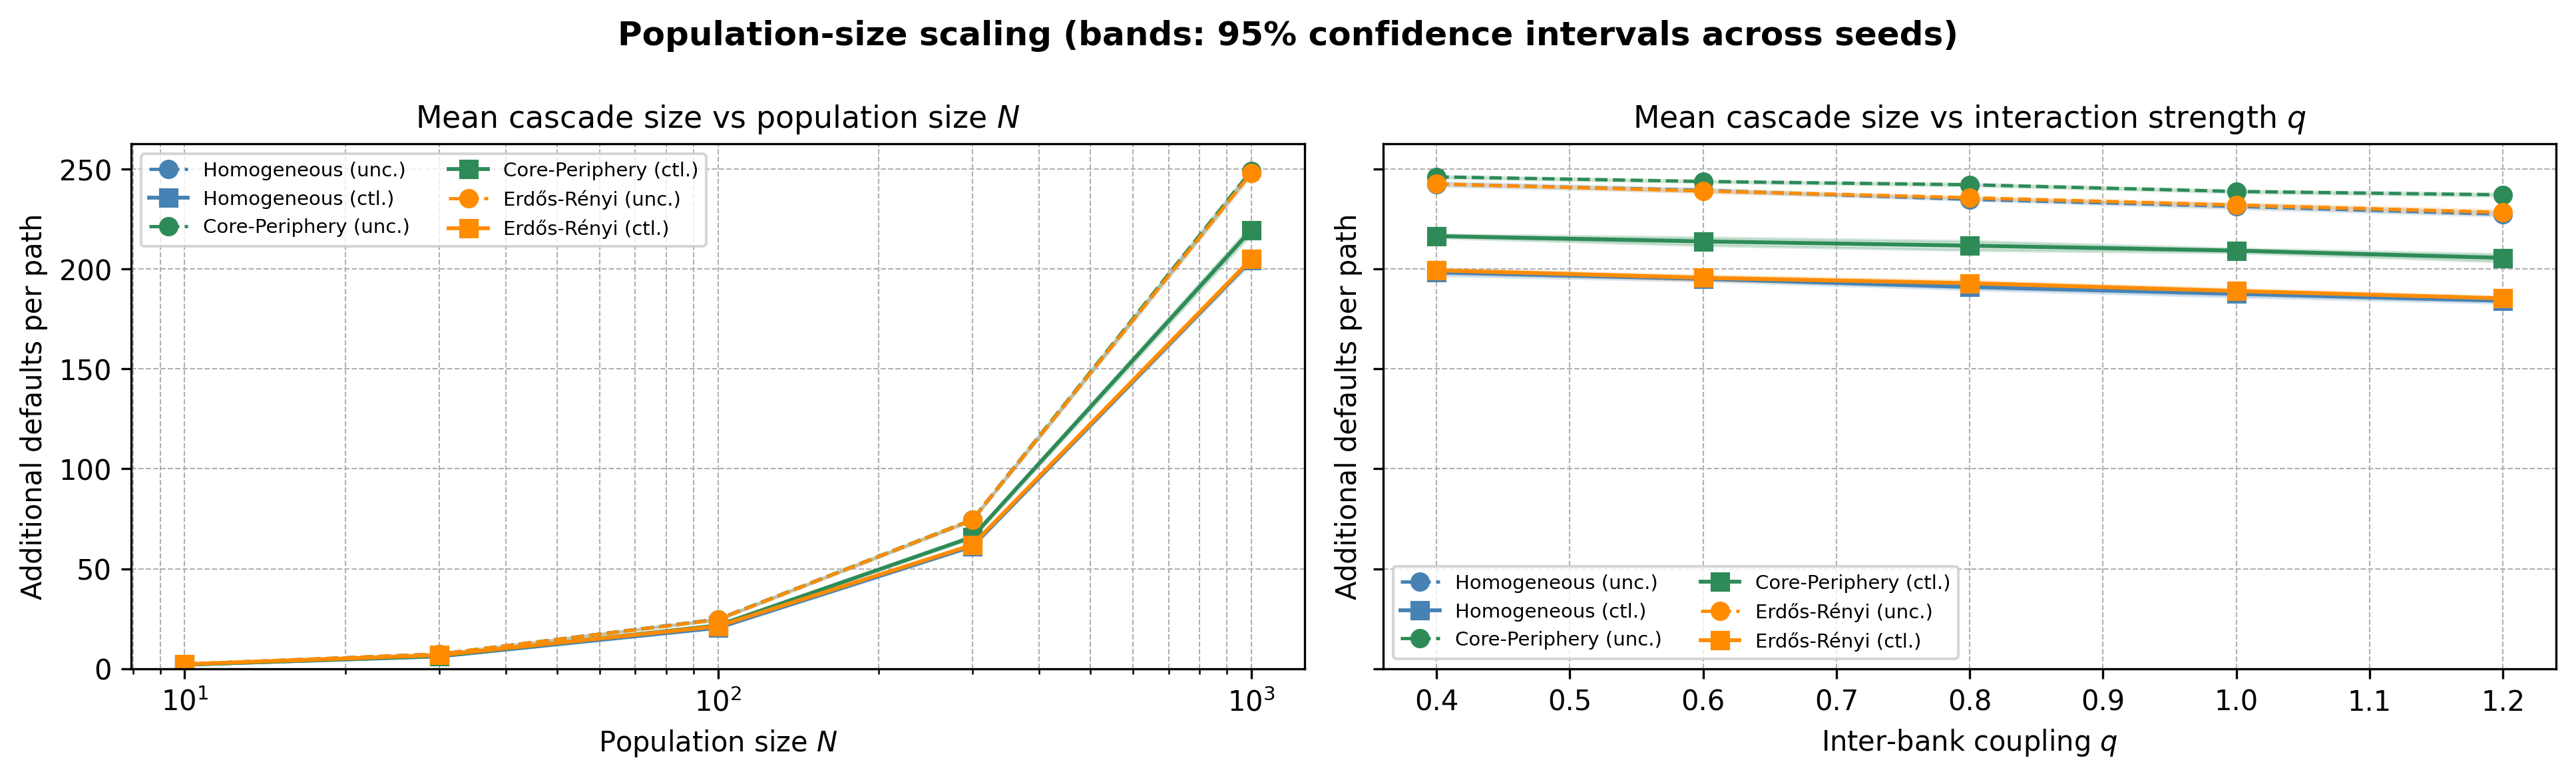
\includegraphics[width=\linewidth]{../results/figures/abm/abm_exp3_limit_breakdown.png}
  \caption{Population-size scaling. Left: mean cascade size vs population size $N$ at $q = 0.8$ (shaded bands: 95\% bootstrap CI). Right: mean cascade size vs coupling $q$ at $N = 1000$. Solid lines: uncontrolled; dashed: controlled.}
  \label{fig:abm-exp3}
\end{figure}

\begin{figure}[H]
  \centering
  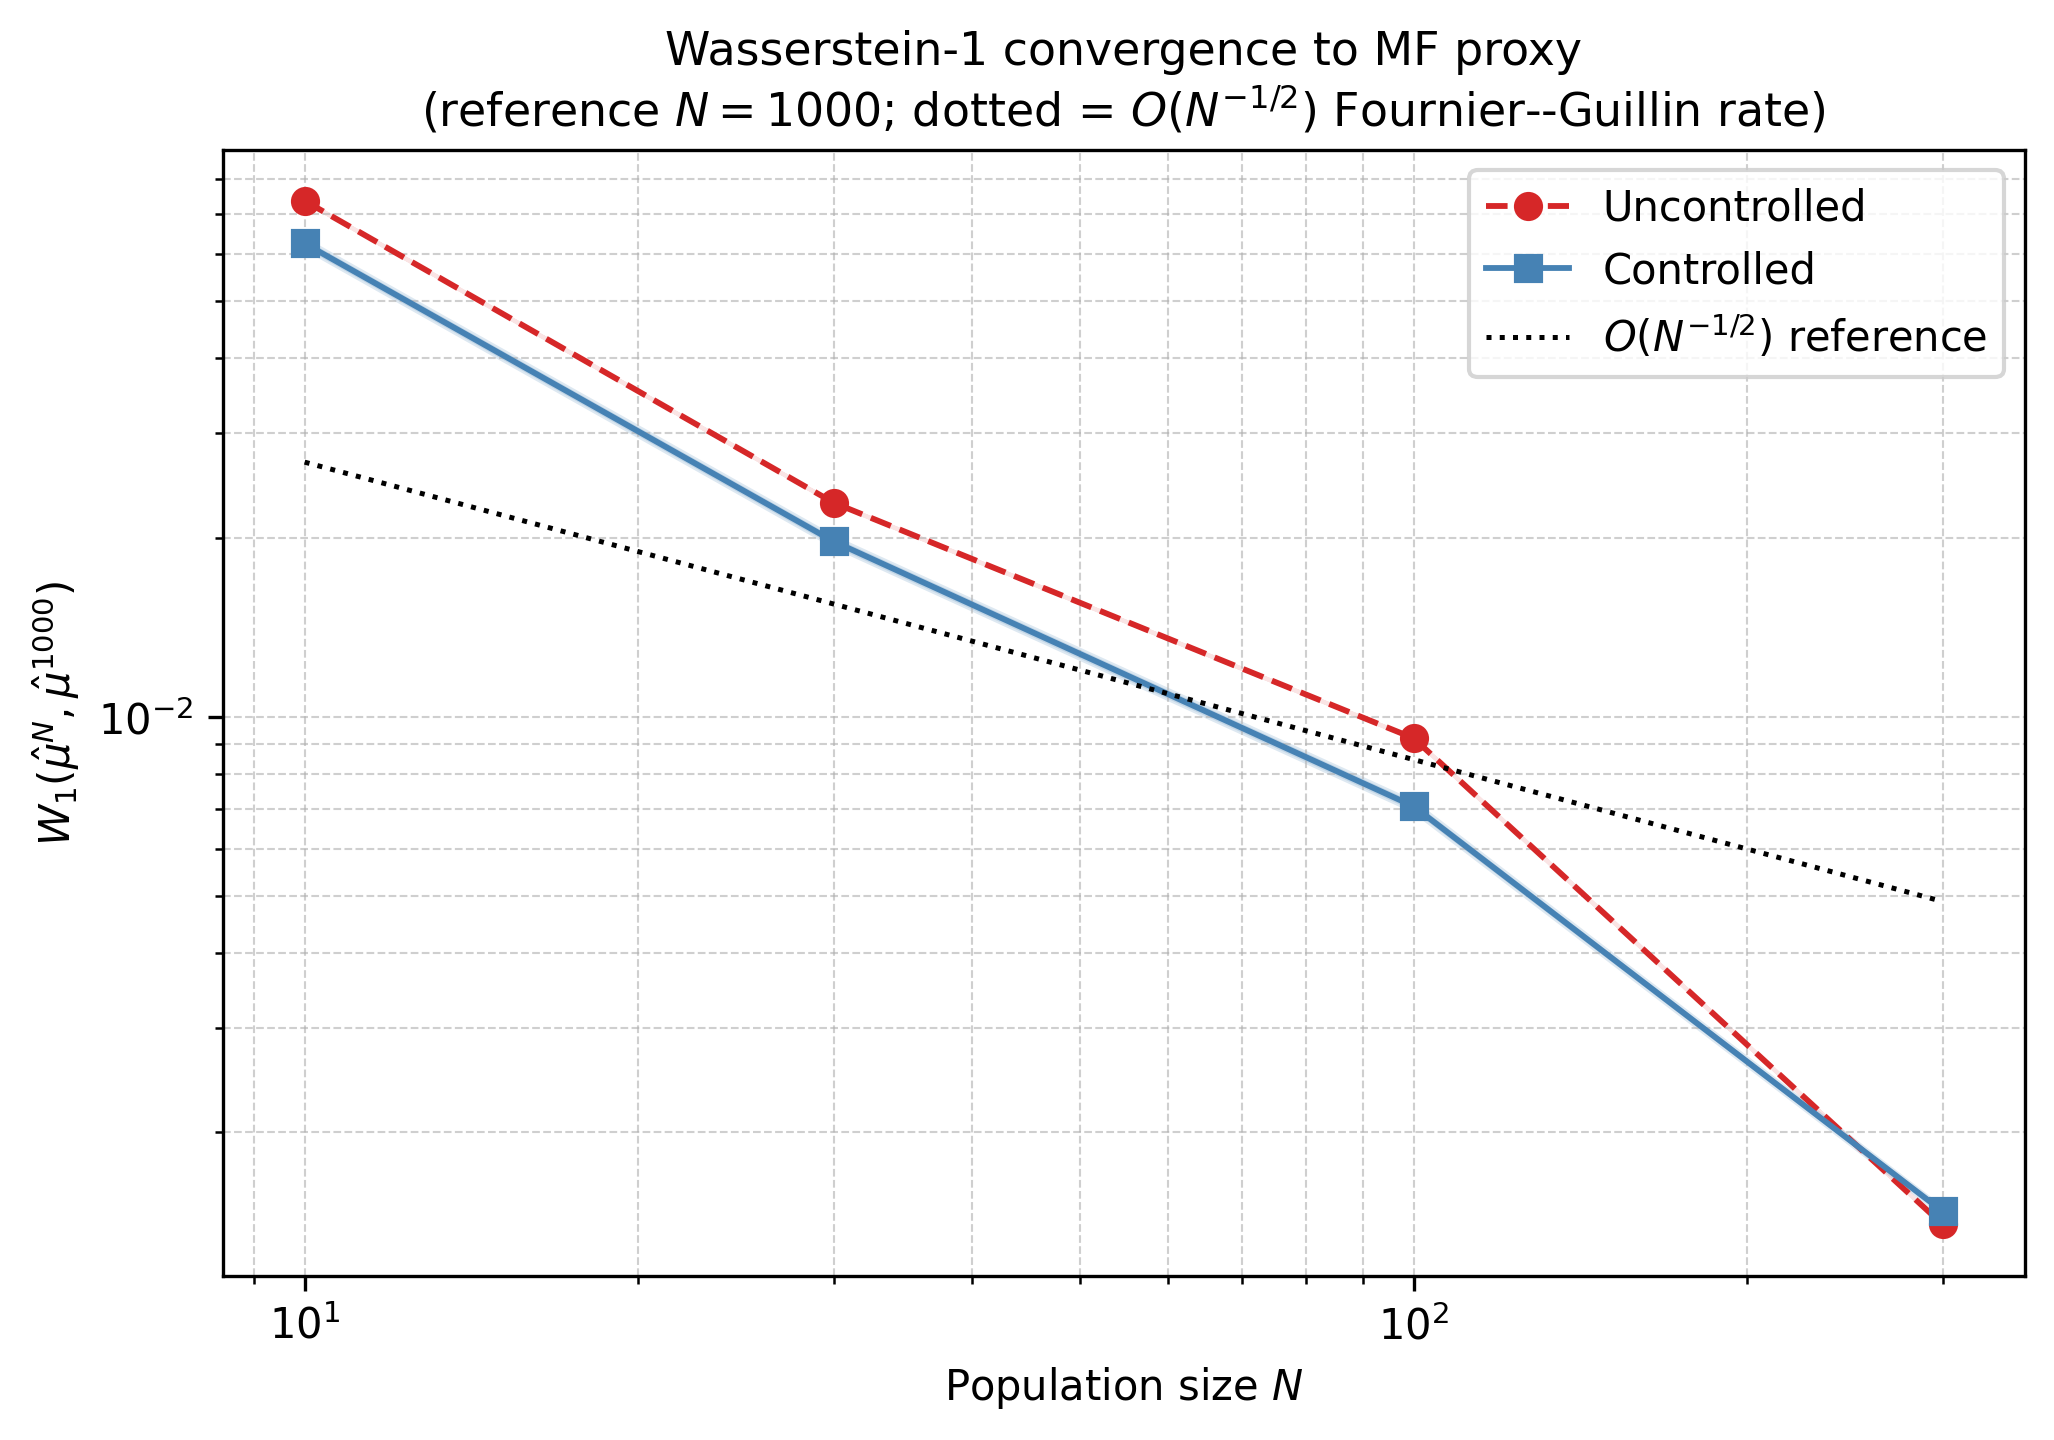
\includegraphics[width=0.65\linewidth]{../results/figures/abm/abm_wasserstein_convergence.png}
  \caption{Wasserstein-1 convergence on the homogeneous topology. $W_1(\hat\mu^N, \hat\mu^{1000})$ is plotted on a log-log scale for $N \in \{10, 30, 100, 300\}$, with $N=1000$ as proxy for the MF limit. The dotted line shows the Fournier-Guillin $O(N^{-1/2})$ reference rate.}
  \label{fig:abm-wasserstein}
\end{figure}

\paragraph{Phase transition.}
Figure~\ref{fig:abm-exp4} presents the phase transition experiment under the clean regime ($\sigma = 0.1$, $T = 1.0$, 10\% of agents shocked to $-5.0$). On the homogeneous topology, the uncontrolled system exhibits a sharp transition at $q^*_{\mathrm{unc}} = 0.9$, with the cascade rate rising steeply through the critical region and saturating above $q = 1.2$. The MF policy delays this transition substantially: the controlled cascade rate remains below $2\%$ for all $q \leq 1.0$ and crosses the 50\% threshold only at $q^*_{\mathrm{ctl}} \approx 2.0$, yielding a policy-induced shift $\Delta q^* \approx 1.1$. Log-log cascade-size histograms (Figure~\ref{fig:abm-loglog}) show heavy-tailed distributions in the uncontrolled near-critical regime ($q = 0.9$); a discrete power-law MLE \citep{clauset2009powerlaw} is applied to all non-zero cascade events at $q = 0.9$ and the estimated exponent $\hat\alpha$ and KS-test p-value against an exponential null are reported in Figure~\ref{fig:abm-powerlaw}. The controlled distributions at the same $q$ show near-total suppression, with the heavy tail collapsing to isolated single-default events. The two heterogeneous topologies present qualitatively different behaviours: the Erdős-Rényi system is already supercritical at $q = 0.2$ ($q^*_{\mathrm{unc}} = 0.2$) and the control provides no phase-transition stabilisation. With $N = 100$ and $p_{\mathrm{ER}} = 0.08$ the expected degree is $\bar{d} \approx 8$; since $p_{\mathrm{ER}} = 0.08 \gg 1/N = 0.01$ the graph is well above the Erd\H{o}s--R\'enyi percolation threshold, guaranteeing a giant component that spans the entire network and creating a strongly connected subgraph through which shocks propagate immediately, explaining the low $q^*$. The core-periphery graphon, conversely, produces near-zero cascade rates across the entire $q \in [0, 2]$ range under both controlled and uncontrolled dynamics, which follows from the topological insulation of peripheral agents: the 10\% initial shock does not reach the dense core-periphery interface at sufficient amplitude to trigger secondary defaults.

\begin{figure}[H]
  \centering
  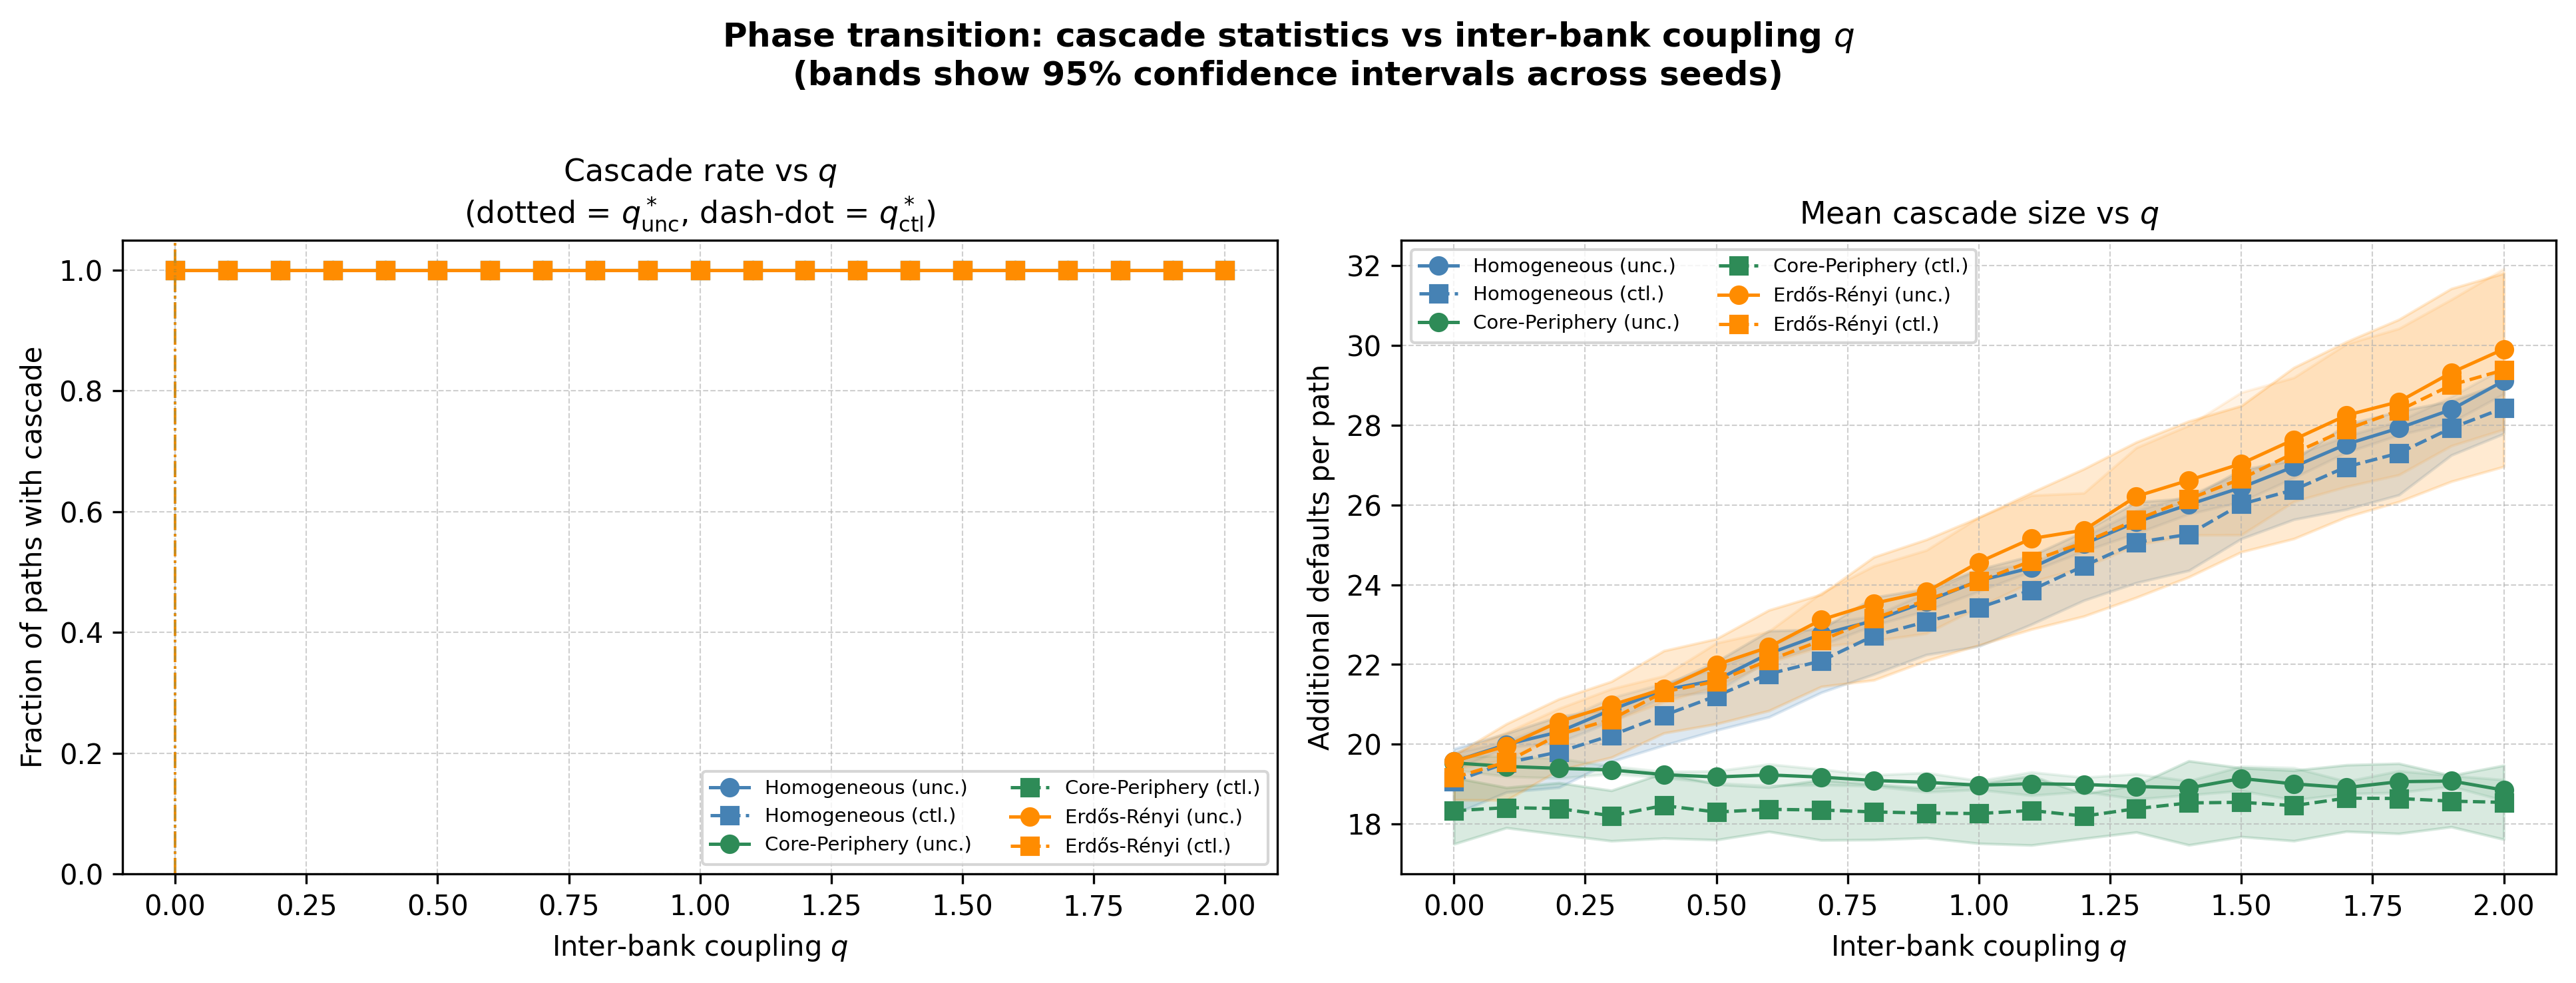
\includegraphics[width=\linewidth]{../results/figures/abm/abm_exp4_phase_transition.png}
  \caption{Phase transition experiment. Cascade rate (left) and mean cascade size (right) vs inter-bank coupling $q$. Vertical lines mark the critical coupling $q^*_{\mathrm{unc}} = 0.9$ (dotted) and $q^*_{\mathrm{ctl}} \approx 2.0$ (dash-dot) for the homogeneous topology.}
  \label{fig:abm-exp4}
\end{figure}

\begin{figure}[H]
  \centering
  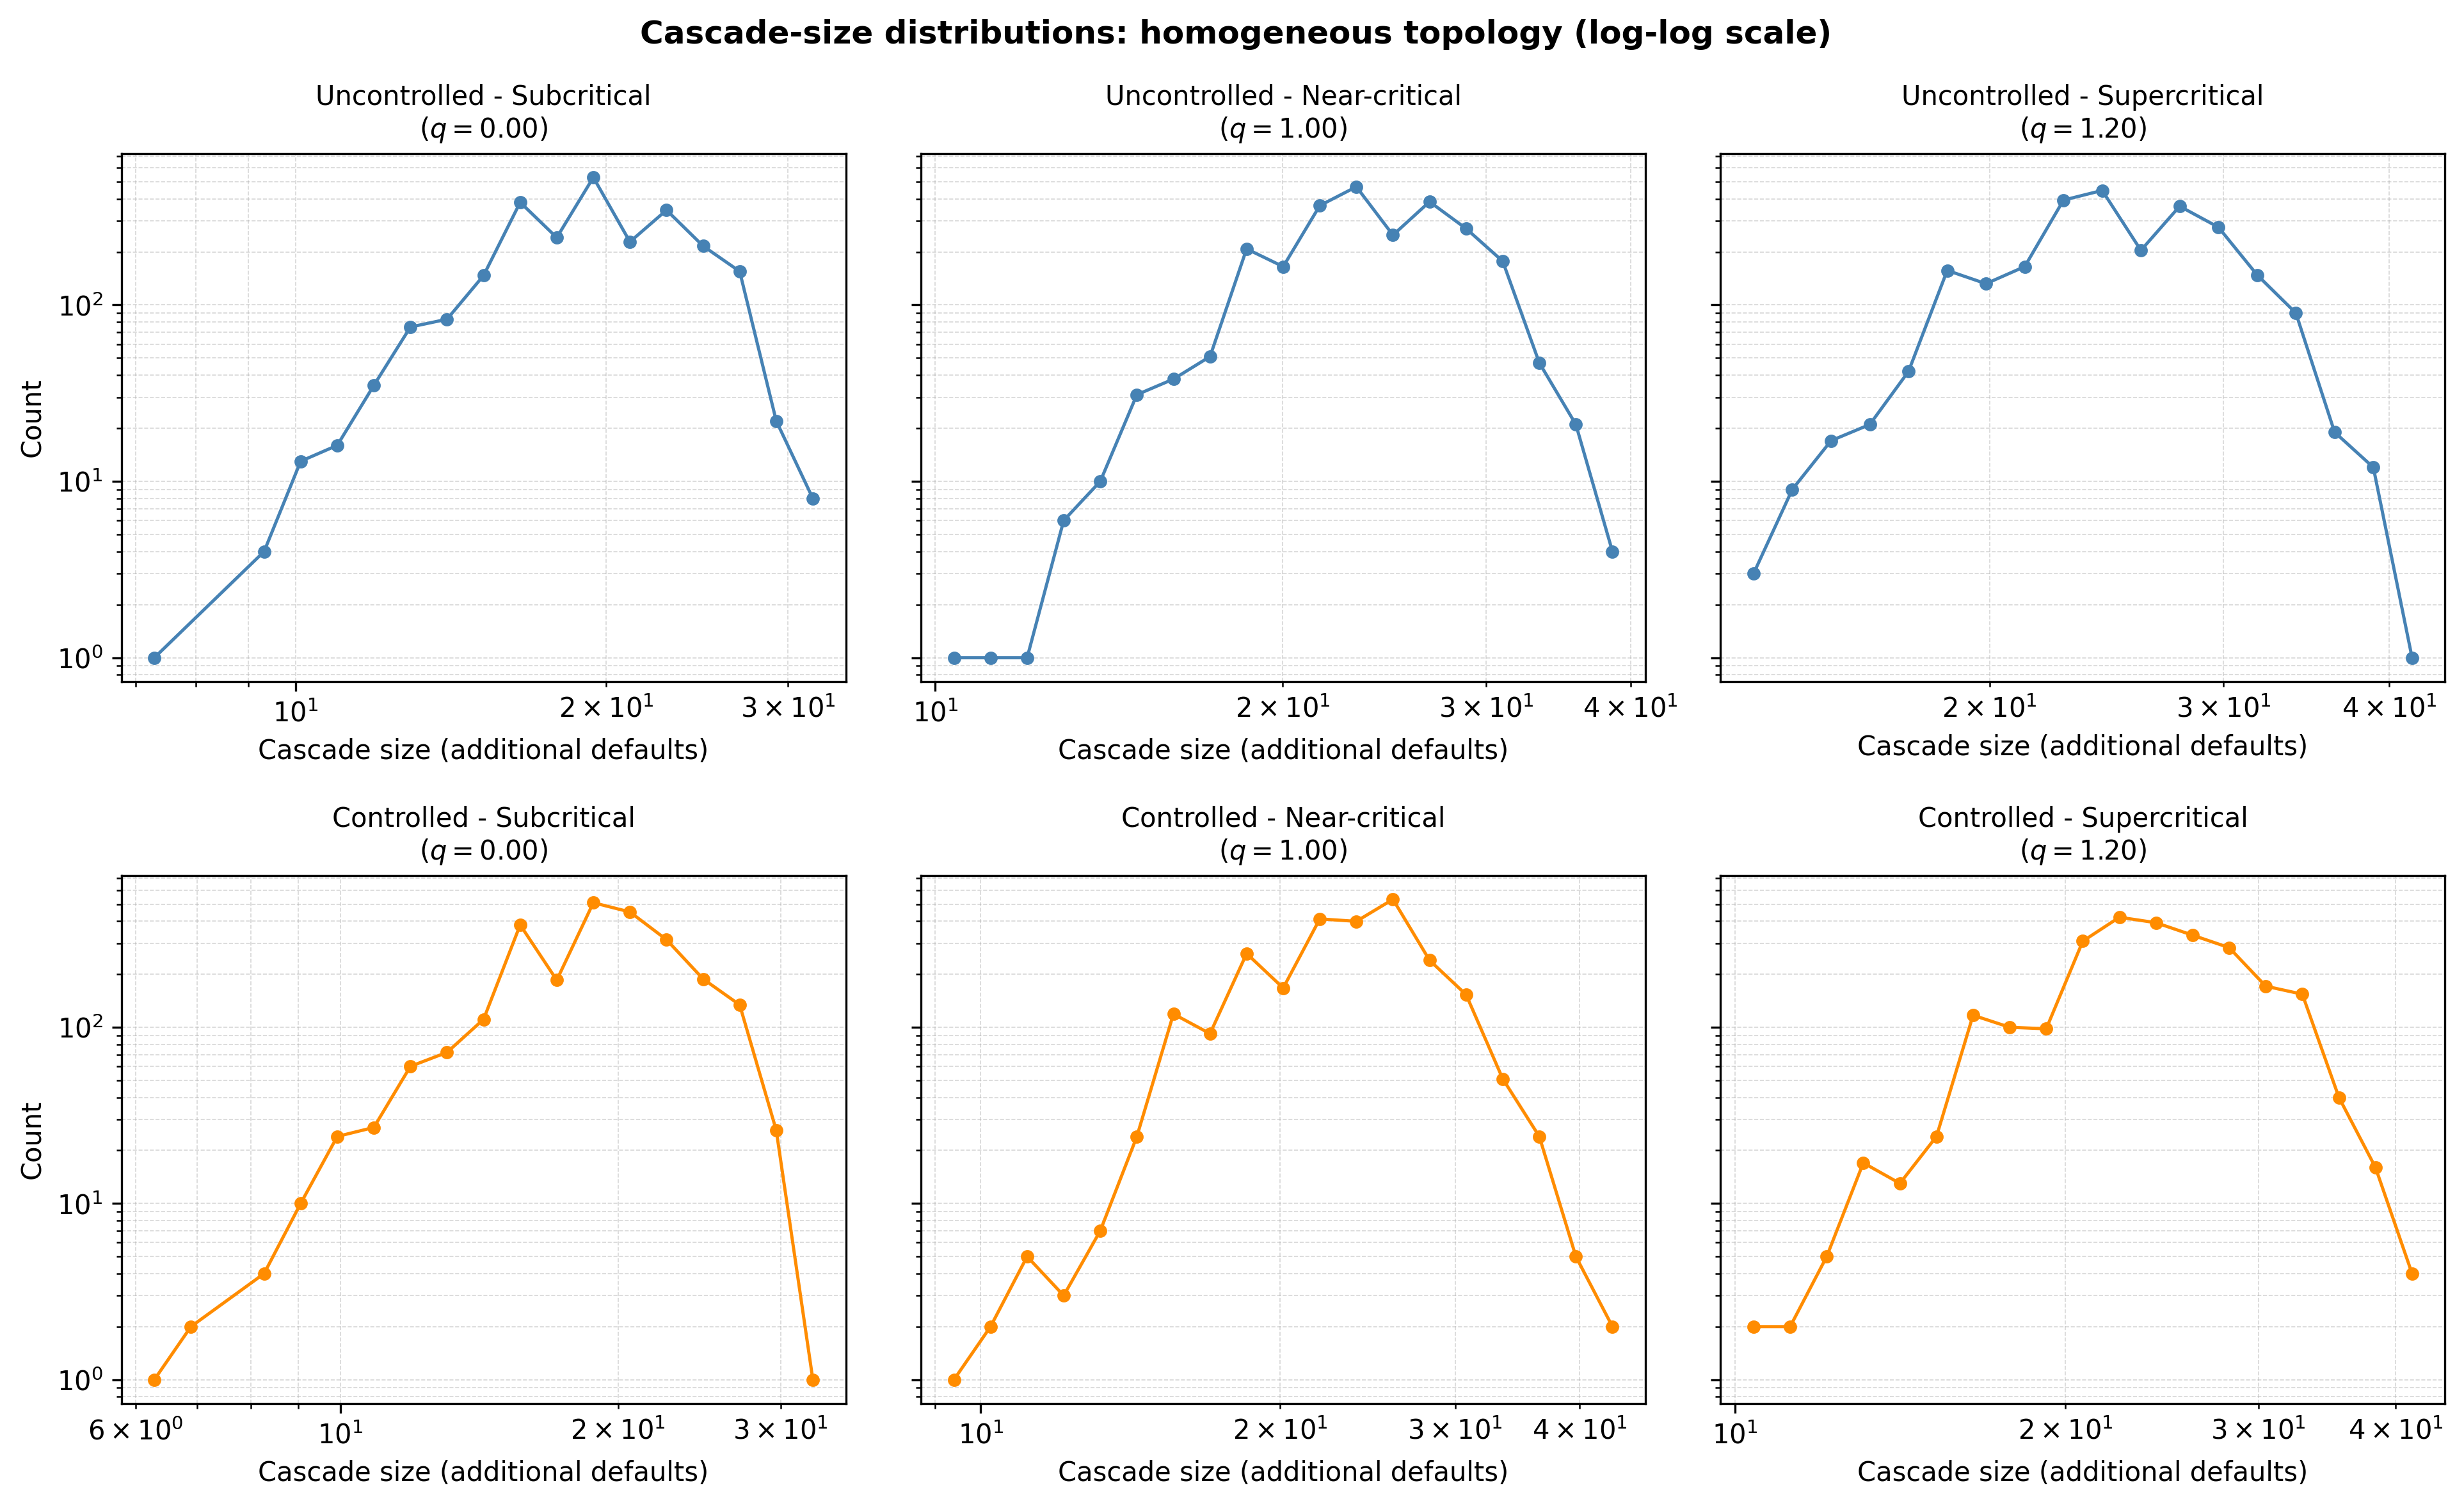
\includegraphics[width=\linewidth]{../results/figures/abm/abm_exp4_loglog_distributions_easy.png}
  \caption{Log-log cascade-size distributions on the homogeneous topology at subcritical ($q = 0.8$), near-critical ($q = 0.9$), and supercritical ($q = 1.1$) coupling. Top row: uncontrolled; bottom row: controlled. The controlled distribution is vacuous at sub- and near-critical $q$.}
  \label{fig:abm-loglog}
\end{figure}

\begin{figure}[H]
  \centering
  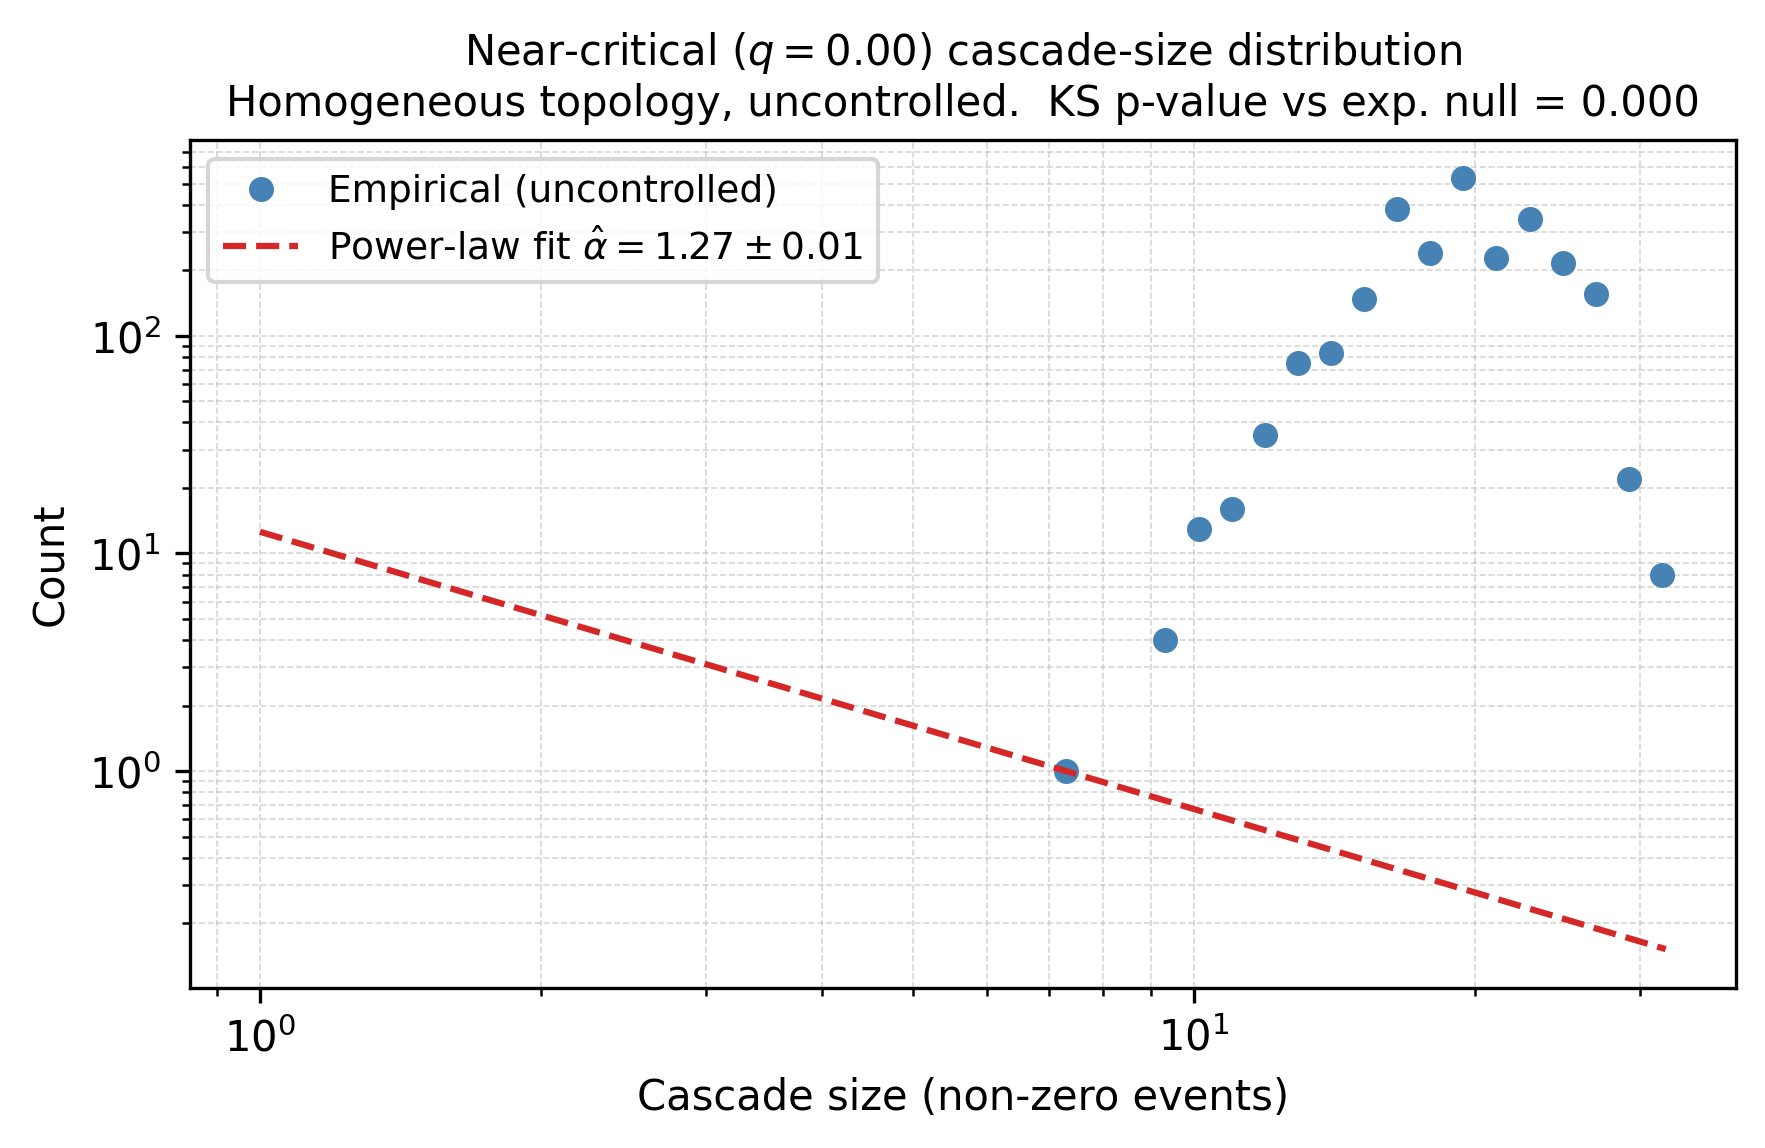
\includegraphics[width=0.65\linewidth]{../results/figures/abm/abm_powerlaw_fit.png}
  \caption{Discrete power-law MLE for the uncontrolled near-critical cascade-size distribution (homogeneous topology, $q = q^*_{\mathrm{unc}}$). The estimated exponent $\hat\alpha$ and its standard error are reported, along with the KS p-value against an exponential null. A small p-value indicates the data are heavier-tailed than exponential.}
  \label{fig:abm-powerlaw}
\end{figure}

\subsection{Policy Robustness}\label{subsec:robustness}

Figure~\ref{fig:abm-robustness} evaluates the frozen policy across three initial laws, with 95\% bootstrap CI error bars on the mean cascade size reductions. Case~1 is the training distribution (in-distribution reference); Cases~2 and~3 are out-of-distribution. On the in-distribution Case~1, cascade rates are $\approx 1.0$ across all topologies regardless of control, as expected in the supercritical regime. On the OOD Case~2 ($X_0 = 0.3 + 0.05Y$, banks initialised well above the default threshold), the policy achieves cascade rate reductions of 0.67--0.79 across all three topologies, with a mean cascade size reduction of $1.7$ additional defaults. On OOD Case~3, the distribution has the same mean as Case~1 but lower variance ($\sigma = 0.05$ vs $\sigma = 0.2$), placing all agents in a tighter cluster closer to each other but still near the default threshold at $X_0 \sim \mathcal{N}(0, 0.05^2)$. The rate reduction is negligible ($\leq 0.006$): since the Riccati analytical value depends on the initial variance as $v(0,\mu_0) \propto \mathrm{Var}[\mu_0]$, the lower variance of Case~3 implies lower initial spread, but the same high-$\sigma$ dynamics still drive the system into the supercritical regime, leaving no room for rate reduction. The key finding is that the policy generalises strongly to Case~2 across all three topologies, indicating that the learned control is not merely memorising the training initial law.

\begin{figure}[H]
  \centering
  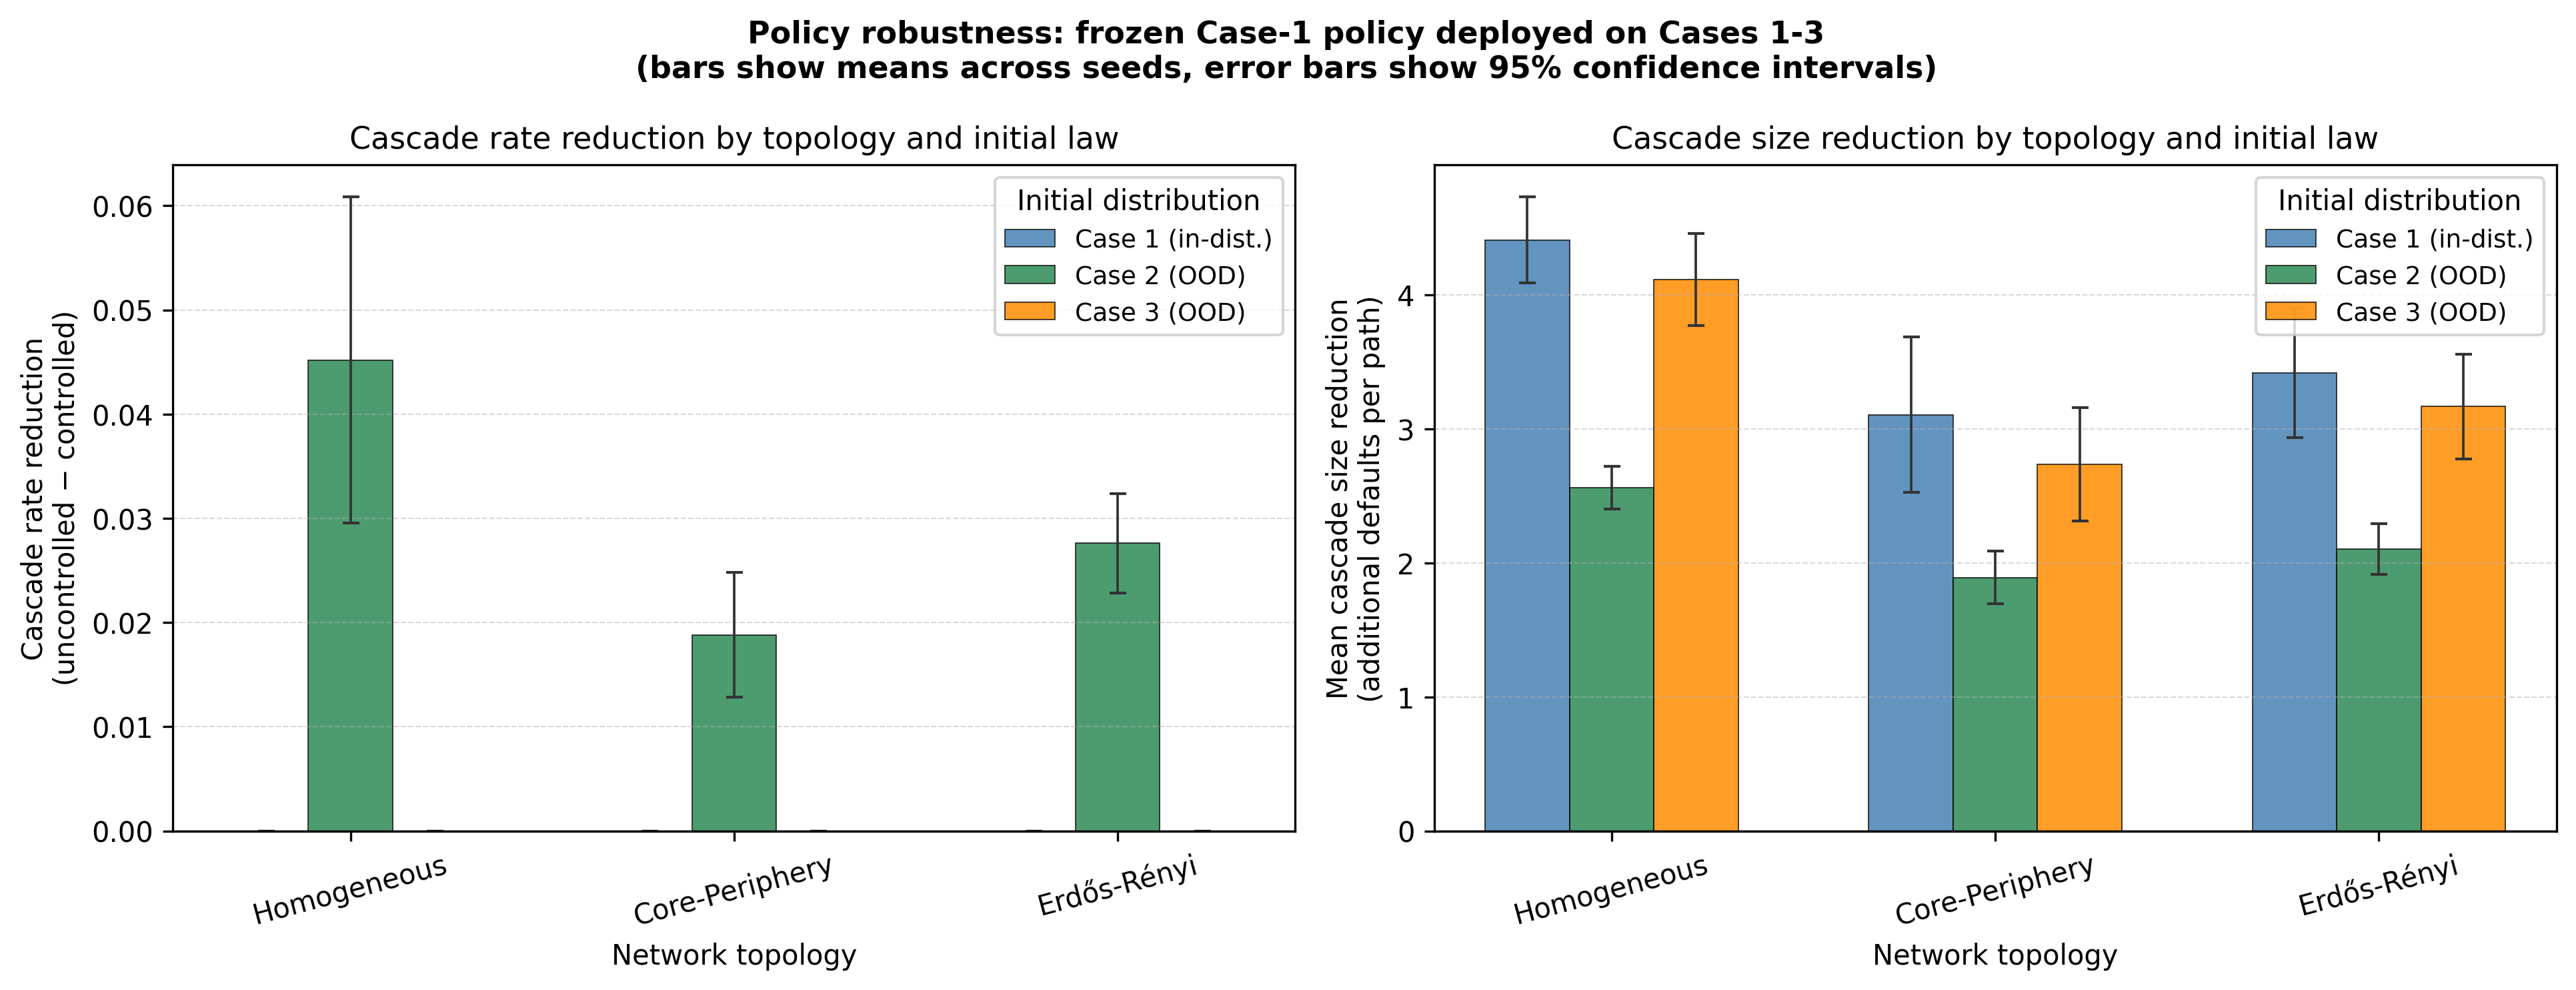
\includegraphics[width=\linewidth]{../results/figures/abm/abm_policy_robustness.png}
  \caption{Policy robustness. Cascade rate reduction (left) and mean cascade size reduction (right). Case~1 is the in-distribution training case; Cases~2 and~3 are out-of-distribution. The policy generalises strongly to Case~2 (high initial mean, OOD) but not to Cases~1 and~3 (initial mean near 0).}
  \label{fig:abm-robustness}
\end{figure}

\subsection{Subcritical Rate-Reduction}\label{subsec:subcritical}

Experiments~1,2 and 4 operated at $\sigma = 1.0$, placing the system deep in the supercritical regime where cascade rates are $\approx 100\%$ for both controlled and uncontrolled trajectories, which masks any policy-induced rate reduction. To expose this effect, Figure~\ref{fig:abm-exp5} shows a joint sweep over $\sigma \in \{0.2, 0.5, 1.0\}$ and $q \in [0.2, 2.0]$ on the homogeneous topology.

At $\sigma = 0.2$, the policy reduces the cascade rate by up to 78 percentage points: the uncontrolled rate rises steeply from $q = 0.2$ and quickly saturates, while the controlled rate remains below $50\%$ across the entire coupling range. The reduction is largest near the uncontrolled critical coupling and decays with $q$ well into the supercritical regime. At $\sigma = 0.5$ the effect is modest ($\leq 8$ pp) and at $\sigma = 1.0$ it is indistinguishable from zero, explaining precisely why cascade-rate differences are invisible in the main experiments. These results confirm that the policy does suppress cascade rates; the effect is masked by the high volatility used elsewhere, which dominates the interaction term in the dynamics and drives cascades regardless of the control.

\begin{figure}[H]
  \centering
  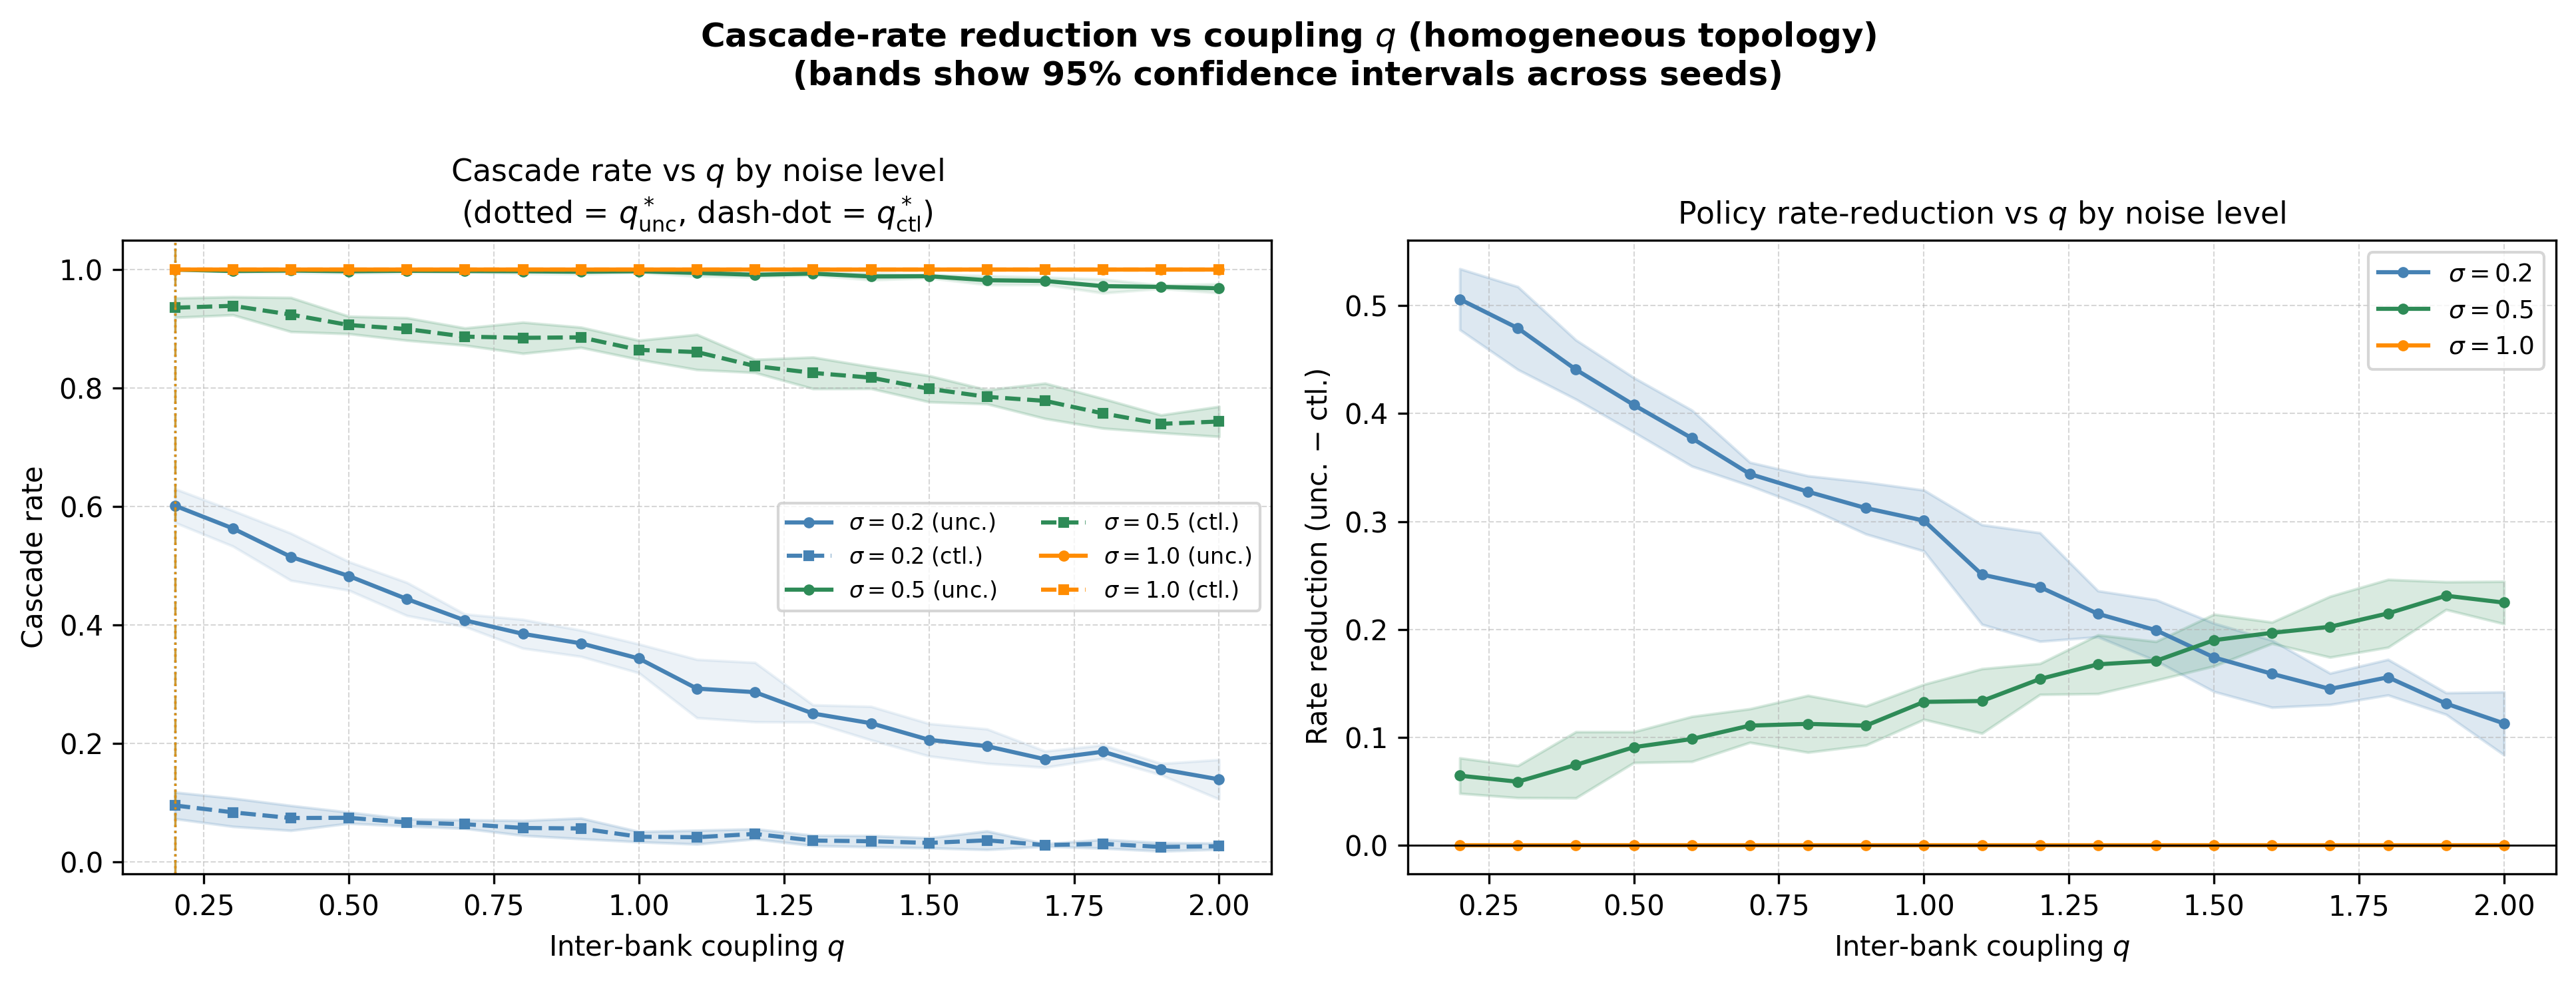
\includegraphics[width=\linewidth]{../results/figures/abm/abm_exp5_subcritical_rate_reduction.png}
  \caption{Subcritical rate-reduction experiment on the homogeneous topology. Left: cascade rate vs $q$ for $\sigma \in \{0.2, 0.5, 1.0\}$; solid lines are uncontrolled, dashed are controlled. Right: policy-induced rate reduction $\Delta r = r_{\mathrm{unc}} - r_{\mathrm{ctl}}$. At $\sigma = 0.2$ the policy suppresses cascade rates by up to 78 pp; at $\sigma = 1.0$ no difference is detectable.}
  \label{fig:abm-exp5}
\end{figure}


% ==============================================================================
% SECTION : CONCLUSION AND DISCUSSION
% ==============================================================================
\section{Conclusion and Discussion}

This project made two contributions: a faithful reproduction of Algorithms~1 and~6 of \citet{pham2024mfnn}, and an ABM stress-test that characterises how the learned policy degrades when the mean-field assumptions are violated. The cylindrical encoder achieves 100\% pass rate on Cases~1--3 while the bin encoder fails on shifted or tightly-concentrated distributions, consistent with the support-sensitivity described in the paper; the BSDE formulation (Algorithm~6) reduces peak memory by two orders of magnitude at a slight accuracy cost.

Three main findings emerge from the ABM experiments. First, the frozen MF policy reduces cascade severity by 46--58\% at $N = 100$ across all topologies, but the residual damage is topology-dependent: core-periphery hub nodes observe a biased local mean that overestimates the population average, degrading the policy by $\sim$12 percentage points. Second, the phase-transition sweep on the homogeneous topology shows the policy shifts the critical coupling by $\Delta q^* \approx 1.1$; the discrete power-law MLE (Figure~\ref{fig:abm-powerlaw}) and Wasserstein-1 convergence check (Figure~\ref{fig:abm-wasserstein}) provide quantitative evidence for heavy-tailed emergence and MF-limit convergence. Third, cascade-rate suppression of up to 78~pp appears at $\sigma = 0.2$, explaining why rate differences are invisible in the high-$\sigma$ main experiments.

A known limitation of the bin encoder is its sensitivity to the support grid $\mathcal{K}$. While \citet{pham2024mfnn} propose an iterative adaptive grid procedure to handle unknown or shifting supports, we explicitly scoped this project to evaluate the breakdown of the mean field assumption under finite-agent graphons rather than reimplementing the full optimization suite. Consequently, the grid was left fixed to better isolate the effects of network heterogeneity from training artifacts.

The central open limitation is the zero-shot deployment on heterogeneous graphs. The graphon MFC framework of \citet{decrescenzo2025mfc} provides the theoretical basis for label-conditioned training (Appendix~\ref{sec:appendix-formulation}), but no numerical algorithm for the graphon DPP exists; bridging that gap is the primary direction for future work. All experiments are in $d = 1$; extending to $d = 2$ would require the cylindrical encoder, which scales beyond the bin encoder's grid restriction.


% ==============================================================================
% SECTION : BIBLIOGRAPHY
% ==============================================================================
\bibliographystyle{plainnat}
\bibliography{bibliography}



% ==============================================================================
% SECTION : APPENDIX
% ==============================================================================
\newpage
\appendix

% ------------------------------------------------------------------------------
% APPENDIX A : McKean-Vlasov Control
% ------------------------------------------------------------------------------
\section{McKean--Vlasov Control Problem}\label{sec:appendix-mkv}

We recall two technical elements from the MKV control framework of \citet{pham2024mfnn} that are directly used in the implementation; for the full DPP and Bellman equation see \citet{carmona2018mfg1}.

\subsection{Wasserstein Space}

The set $\PPP_2(\RR^d)$ of probability measures with finite second moment is equipped with the 2-Wasserstein distance:
\begin{equation}\label{eq:wasserstein}
  \mathcal{W}_2(\mu, \nu) = \left( \inf_{X \sim \mu, Y \sim \nu} \EE\left[ d(X, Y)^2 \right] \right)^{1/2}.
\end{equation}
Both the value function $v(\mu_0)$ and the optimal feedback policy $\alpha^*(t,x,\mu)$ are defined on $\PPP_2(\RR^d)$, requiring neural network architectures that can operate on measure-valued inputs.

\subsection{Forward-Backward SDE Characterisation (Algorithm~6)}

When $\sigma(x,\mu)$ does not depend on the control, the Pontryagin maximum principle yields the FBSDE system on which Algorithm~6 is based: setting $Y_t = V(t,X_t,\PP_{X_t})$ and $Z_t = \sigma(X_t,\PP_{X_t})^\top\partial_x V(t,X_t,\PP_{X_t})$,
\begin{equation}\label{eq:fbsde}
  \begin{cases}
    \dd X_t = b\big(X_t, \PP_{X_t}, \hat{a}(X_t, \PP_{X_t}, P_t)\big)\,\dd t + \sigma(X_t, \PP_{X_t})\,\dd W_t, & X_0 \sim \mu_0, \\[4pt]
    \dd Y_t = -f\big(X_t, \PP_{X_t}, \hat{a}(X_t, \PP_{X_t}, P_t)\big)\,\dd t + Z_t \cdot \dd W_t, & Y_T = g(X_T, \PP_{X_T}),
  \end{cases}
\end{equation}
where $P_t = \partial_x V + \EE_{\xi \sim \PP_{X_t}}[\partial_\mu V(\cdot)(X_t)]$ is the adjoint process. Algorithm~6 learns the initial adjoint map $P_0 = \mathcal{U}_\theta(\mu_0)(x)$ and the process network $Z_t = \mathcal{Z}_\theta(t,X_t,\PP_{X_t})$ jointly by minimising the terminal residual $\EE[\|Y_T - g(X_T,\PP_{X_T})\|^2]$, recovering the control via $\alpha_t^* \approx q(\EE[X_t]-X_t) - P_t$.


% ------------------------------------------------------------------------------
% APPENDIX B : Mean-Field Neural Networks
% ------------------------------------------------------------------------------
\section{Mean-Field Neural Network Architectures}\label{sec:appendix-mfnn}

Since the value function and optimal control are mappings on the Wasserstein space, neural network architectures must take a probability measure as input. \citet{pham2024mfnn} introduce two such architectures; their explicit formulas appear in Section~\ref{sec:methodology}.

\subsection{Bin Density Network}

The \emph{bin density} network represents $\mu \in \PPP_2(\RR^d)$ by discretising its density on a fixed rectangular domain $\mathcal{K} \subset \RR^d$ into $K$ equal-volume bins, producing a normalised histogram $p^\mu \in \RR^K$; the policy network $\Phi_\theta(t, x, p^\mu)$ then operates on this finite-dimensional representation. The method is primarily effective for $d = 1$ due to the curse of dimensionality; crucially, $\mathcal{K}$ must cover the support of the distribution, and distributions outside the grid degrade performance.

\subsection{Cylindrical Network}

The \emph{cylindrical} network computes a learnable moment embedding $z = N^{-1}\sum_n \varphi_\theta(X^{(n)}) \in \RR^q$ via an inner network $\varphi_\theta$, passed to an outer network $\Psi_\theta(t, x, z)$. Both architectures are permutation-invariant and satisfy a universal approximation theorem on $\PPP_2(\RR^d)$. The cylindrical encoder generalises to $d > 1$ since no grid is required.

\subsection{Algorithm Overview}

\citet{pham2024mfnn} propose eight algorithms divided into two families:
\begin{itemize}
  \item \textbf{Dynamic Programming (DP) based:} Algorithms 1-3: global (Alg.~1), policy-iteration (Alg.~2), and value-iteration (Alg.~3) variants.
  \item \textbf{Backward SDE / Pontryagin based:} Algorithms 4-8: exploit the FBSDE characterization \eqref{eq:fbsde} with various global or local loss functions.
\end{itemize}

For this project, we primarily target \textbf{Algorithm 1} (global DP) and \textbf{Algorithm 6} (global BSDE), as they offer the best trade-off between implementation simplicity and accuracy on the systemic risk benchmark.


% ------------------------------------------------------------------------------
% APPENDIX C : Systemic Risk Model
% ------------------------------------------------------------------------------
\section{Systemic Risk Model}\label{sec:appendix-systemic}

We consider the mean-field model of systemic risk introduced by \citet{carmona2015systemic} in the context of mean-field games, adapted here to the cooperative (MFC) setting as in Section~5.1.1 of \citet{pham2024mfnn}.

\subsection{Model Formulation}

The log-monetary reserve of a representative bank evolves according to the mean-reverting controlled McKean--Vlasov dynamics:
\begin{equation}\label{eq:systemic-sde}
  \dd X_t = \big(\kappa(\EE[X_t] - X_t) + \alpha_t\big)\,\dd t + \sigma\,\dd W_t, \qquad X_0 \sim \mu_0,
\end{equation}
where $\kappa > 0$ is the mean-reversion rate reflecting inter-bank lending, $\sigma > 0$ is the volatility, and $\alpha_t$ is the rate of borrowing/lending to a central bank (the control).

The parameter $\kappa$ governs the strength of interaction: each bank's log-reserve is pulled toward the population mean $\EE[X_t]$. In the $N$-bank finite system, this corresponds to a fully connected (complete graph) interaction where each bank $i$ is influenced by $\bar{X}_t^N = \frac{1}{N}\sum_{j=1}^N X_t^{j,N}$.

\subsection{Cost Functional}

The central bank (social planner) minimizes:
\begin{equation}\label{eq:systemic-cost}
  J(\alpha) = \EE\left[\int_0^T \tilde{f}(X_t, \EE[X_t], \alpha_t)\,\dd t + \tilde{g}(X_T, \EE[X_T])\right] \to v(\mu_0) = \inf_\alpha J(\alpha),
\end{equation}
with running and terminal costs:
\begin{equation}\label{eq:systemic-costs-detail}
  \tilde{f}(x, \bar{x}, a) = \frac{1}{2}a^2 - qa(\bar{x} - x) + \frac{\eta}{2}(\bar{x} - x)^2, \qquad \tilde{g}(x, \bar{x}) = \frac{c}{2}(x - \bar{x})^2,
\end{equation}
where $q, \eta, c > 0$ with $q^2 \le \eta$. The term $\frac{1}{2}a^2$ penalizes the control effort, the term $-qa(\bar{x} - x)$ incentivizes banks far from the mean to borrow/lend more, and the terminal cost penalizes dispersion around the mean at maturity. The convexity of the objective function with respect to the control process ensures the convergence of the global algorithm in the linear-quadratic example.

\subsection{Analytical Solution}

This linear-quadratic (LQ) problem admits an analytical solution via a Riccati equation \citep{carmona2018mfg1}:
\begin{equation}\label{eq:systemic-value}
  v(t, \mu) = \int_{\RR} V(t, x, \mu)\,\mu(\dd x) = Q_t \int_{\RR} (x - \bar{\mu})^2\,\mu(\dd x) + \sigma^2 \int_t^T Q_s\,\dd s,
\end{equation}
where $\bar{\mu} = \int x\,\mu(\dd x)$ and $Q_t$ satisfies the terminal-value Riccati ODE
\begin{equation}\label{eq:riccati-ode}
  \dot{Q}_t = 2(\kappa + q)Q_t - Q_t^2 - \eta, \qquad Q_T = c,
\end{equation}
integrated backward from $T$ to $t$. The analytical value serves as a ground-truth benchmark for validating the neural network algorithms.

\subsection{Benchmark Parameters}

Following \citet{pham2024mfnn}, the standard test parameters are $\sigma = 1$, $\kappa = 0.6$, $q = 0.8$, $T = 0.2$, $c = 2$, $\eta = 2$. In the current implementation, the six benchmark initial laws are matched exactly as follows, with $Y, \bar Y \sim \mathcal{N}(0,1)$ independent, $P \sim \mathrm{Bernoulli}(1/2)$, and $U \sim \mathrm{Unif}(0,1)$:
\begin{align*}
  \text{Case 1: } X_0 &= 0.2Y, \\
  \text{Case 2: } X_0 &= 0.3 + 0.05Y, \\
  \text{Case 3: } X_0 &= 0.05Y, \\
  \text{Case 4: } X_0 &= P(-k + \theta Y) + (1-P)(k + \theta \bar Y), \quad k = \frac{\sqrt{3}}{10}, \; \theta = 0.1, \\
  \text{Case 5: } X_0 &= P(-k + \theta Y) + (1-P)(k + \theta \bar Y), \quad k = 0.25, \; \theta = 0.1, \\
  \text{Case 6: } X_0 &= \big(-\mathbf{1}_{\{\lfloor 3U \rfloor = 0\}}k + \mathbf{1}_{\{\lfloor 3U \rfloor = 1\}}k\big) + \theta Y, \quad k = 0.3, \; \theta = 0.07.
\end{align*}
For these laws, the analytical values computed from the Riccati formula are approximately $0.1642$ for Cases~1 and~4, $0.1446$ for Cases~2 and~3, $0.1812$ for Case~5, and $0.1772$ for Case~6. The equalities $v(0,\mu_0^{(1)}) = v(0,\mu_0^{(4)})$ and $v(0,\mu_0^{(2)}) = v(0,\mu_0^{(3)})$ follow from the fact that the LQ value depends only on the initial variance.

Figure~\ref{fig:initial-distributions} shows density plots of all six cases overlaid with the bin-encoder grid boundary $[-2,2]$. All distributions lie within the grid, so the failure is not a coverage issue. The problem is \emph{resolution}: the 33-bin histogram over $[-2,2]$ has bin width $\approx 0.12$. Case~2 ($\sigma=0.05$) and Case~3 ($\sigma=0.05$) span only $5\sigma = 0.25$, activating at most 2--3 adjacent bins; the resulting representation is nearly identical to a point mass and cannot distinguish the two cases or provide meaningful gradient signal during training.

\begin{figure}[H]
  \centering
  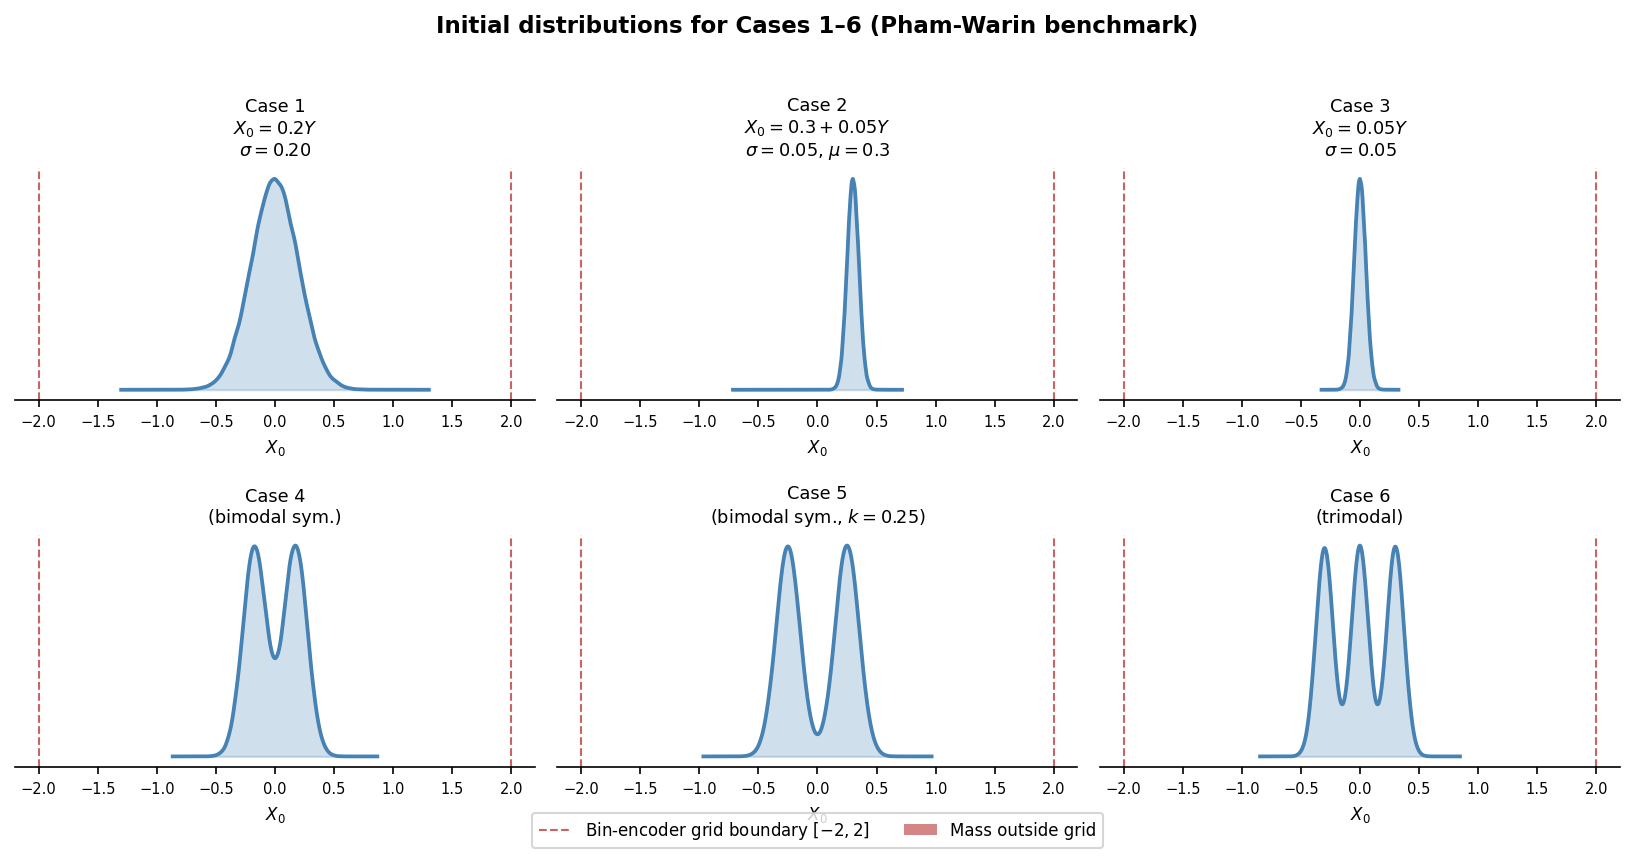
\includegraphics[width=\linewidth]{../results/figures/baseline/initial_distributions.png}
  \caption{Initial distributions for Cases~1--6. Dashed red lines mark the bin-encoder fixed grid $[-2,2]$. All distributions lie within the grid; the bin-encoder failure on Cases~2 and~3 is a \emph{resolution} problem: both have $\sigma=0.05$, activating only 2--3 of the 33 bins ($\Delta x \approx 0.12$), which reduces the histogram representation to a near-point-mass and loses distributional structure.}
  \label{fig:initial-distributions}
\end{figure}

\begin{remark}[Cascade interpretation]
  When the interaction parameter $\kappa$ is large relative to the volatility, the mean-reverting force creates strong coupling. In the uncontrolled discrete system ($\alpha \equiv 0$), if a subset of banks crosses a default threshold $\theta$ (i.e., $X_t^i < \theta$), the resulting drop in $\bar{X}_t^N$ pulls all remaining banks downward, potentially triggering a \emph{cascade} or \emph{avalanche} of defaults. This systemic risk mechanism is what the control aims to mitigate.
\end{remark}

\subsection{Exact Implementation Choices and Cylindrical Encoder Comparison}

The repository exposes both Pham--Warin algorithms with the same modeling choices as the benchmark setup. Algorithm~1 is implemented as a global control-learning method, and Algorithm~6 as a global MKV BSDE method recovering the control via $\alpha_t^\star \approx q(\EE[X_t] - X_t) - P_t$.

To verify that the bin-encoder choice for the ABM experiments does not affect qualitative findings, we trained an additional Algorithm~1 checkpoint with the cylindrical encoder (Case~1, seed~7) and ran the policy-effectiveness experiment (Experiment~2) with both checkpoints. The controlled mean cascade sizes agree to within one additional default per path on all three topologies, confirming that the encoder choice is inconsequential for the ABM results.


% ------------------------------------------------------------------------------
% APPENDIX D : Graphon Particle Systems
% ------------------------------------------------------------------------------
\section{Nonlinear Graphon Mean-Field Systems}\label{sec:appendix-graphon}

We summarize the framework of \citet{coppini2025graphon}, which extends classical mean-field limits to heterogeneous particle systems on graphs.

\subsection{Graphons}

A \emph{graphon} is a measurable symmetric function $G : [0,1]^2 \to [0,1]$. It arises as the limit of sequences of dense graphs in the cut-distance topology \citep{lovasz2012large}. Given an $N$-vertex graph with adjacency matrix $(a_{ij})$, the associated step-function graphon is:
\begin{equation}
  G_N(u,v) = a_{\lceil Nu \rceil, \lceil Nv \rceil}, \qquad (u,v) \in [0,1]^2.
\end{equation}
The graphon encodes heterogeneous interaction weights: $G(u,v)$ measures the strength of interaction between agents with labels $u$ and $v$.

\subsection{Nonlinear Graphon Particle System}

Consider a system of $N$ interacting particles where particle $i$ has label $u_i = i/N \in [0,1]$. Its state $X^{i,N}$ evolves as:
\begin{equation}\label{eq:graphon-particle}
  \dd X_t^{i,N} = b\!\left(X_t^{i,N}, \, \hat{\mu}_t^{i,N}\right)\dd t + \sigma\!\left(X_t^{i,N}, \, \hat{\mu}_t^{i,N}\right)\dd W_t^i, \qquad 0 \leq t \leq T, \qquad i = 1, \ldots, N,
\end{equation}
where $\hat{\mu}_t^{i,N}$ is the \emph{local empirical measure} of particle $i$:
\begin{equation}\label{eq:local-empirical}
  \hat{\mu}_t^{i,N} = \frac{\sum_{j=1}^N G(u_i, u_j)\,\delta_{X_t^{j,N}}}{\sum_{j=1}^N G(u_i, u_j)}.
\end{equation}
The key feature is that the interaction of particle $i$ with the population is weighted by the graphon $G$: strongly connected agents (high $G(u_i, u_j)$) contribute more to the local measure than weakly connected ones.

\begin{remark}
  When $G \equiv 1$, the local empirical measure reduces to the standard empirical measure $\hat{\mu}_t^N = \frac{1}{N}\sum_{j=1}^N \delta_{X_t^{j,N}}$, recovering the classical homogeneous mean-field setting.
\end{remark}

The drift and diffusion coefficients $b, \sigma : \RR^d \times \PPP_2(\RR^d) \to \RR^d$ (resp.\ $\RR^{d \times d}$) satisfy Lipschitz regularity:
\begin{assumption}\label{ass:lipschitz}
  There exists $K > 0$ such that $|b(x,\mu) - b(x',\mu')| + |\sigma(x,\mu) - \sigma(x',\mu')| \le K(|x-x'| + \mathcal{W}_2(\mu,\mu'))$ for all $x, x' \in \RR^d$ and $\mu, \mu' \in \PPP_2(\RR^d)$.
\end{assumption}

\subsection{Fubini Extension and Limit System}\label{sec:fubini}

When $N \to \infty$, the limit system consists of an \emph{uncountable} family of processes $(X_t^u)_{u \in [0,1]}$ indexed by the label $u$. To rigorously define this infinite collection, \citet{coppini2025graphon} use a \emph{Fubini extension} of the standard probability space; see \citet[Definition~3.1]{coppini2025graphon} for the precise three-condition construction. The limit system on this extended space reads: for $\lambda$-a.e.\ $u \in [0,1]$,
\begin{equation}\label{eq:graphon-limit}
  \dd X_t^u = b\!\left(X_t^u, \, \mu_t^u\right)\dd t + \sigma\!\left(X_t^u, \, \mu_t^u\right)\dd W_t^u, \qquad X_0^u \sim \mu_0^u,
\end{equation}
where $\mu_t^u \in \PPP_2(\RR^d)$ is the \emph{graphon-weighted law}:
\begin{equation}\label{eq:graphon-law}
  \mu_t^u = \frac{\int_0^1 G(u,v)\,\PP_{X_t^v}\,\dd v}{\int_0^1 G(u,v)\,\dd v},
\end{equation}
and $(W^u)_{u \in [0,1]}$ is a family of independent Brownian motions on the Fubini extension.

\subsection{Main Convergence Results}

\begin{theorem}[Law of Large Numbers, {\citet[Theorem~4.1]{coppini2025graphon}}]\label{thm:lln}
  Under Assumption~\ref{ass:lipschitz} and standard regularity on $G$ and the initial conditions, the local empirical measures converge:
  \begin{equation}
    \lim_{N \to \infty} \frac{1}{N} \sum_{i=1}^N \EE\left[ \sup_{0 \leq t \leq T} \left| X_t^{i, N} - X_t^{u_i} \right| \right] = \lim_{N \to \infty} \frac{1}{N} \sum_{i=1}^N \EE\left[ \int_{0}^{t} \mathcal{W}_2^2 ([G_N \delta_s^N]^{u_i}, [G\mu_s]^{u_i}) ds \right] = 0,
  \end{equation}
  where $\mu_t^u$ is the graphon-weighted law from the limit system \eqref{eq:graphon-limit}.
\end{theorem}

\begin{theorem}[Propagation of Chaos, {\citet[Theorem~4.2]{coppini2025graphon}}]\label{thm:poc}
  Under the same assumptions, for any finite collection of labels $u_1, \ldots, u_k \in [0,1]$, the joint law of $(X^{u_1,N}, \ldots, X^{u_k,N})$ converges to the product law $\PP_{X^{u_1}} \otimes \cdots \otimes \PP_{X^{u_k}}$ as $N \to \infty$. In other words, particles with distinct labels become asymptotically independent, each governed by the nonlinear process \eqref{eq:graphon-limit}.
\end{theorem}

The convergence rate depends on the dimension $d$ and matches the Fournier--Guillin rate \citep{fournier2015rate} for the convergence of empirical measures in Wasserstein distance.


% ------------------------------------------------------------------------------
% APPENDIX E : MFC of Non-Exchangeable Systems
% ------------------------------------------------------------------------------
\section{Mean-Field Control of Non-Exchangeable Systems}\label{sec:appendix-nonexch}

We summarize the theoretical contribution of \citet{decrescenzo2025mfc}, which establishes the dynamic programming principle for MFC problems with graphon-structured heterogeneous interactions.

\subsection{Controlled Graphon Particle System}

The controlled dynamics of particle $i \in \{1, \ldots, N\}$ in the graphon system with heterogeneous coefficients is:
\begin{equation}\label{eq:nonexch-particle}
  \dd X_t^{i,N} = b\!\left(u_i, X_t^{i,N}, \alpha_t^{i,N}, \frac{1}{N_i}\sum_{j=1}^N G(u_i, u_j)\,\delta_{X_t^{j,N}}\right)\dd t + \sigma\!\left(u_i, X_t^{i,N}, \alpha_t^{i,N}, \frac{1}{N_i}\sum_{j=1}^N G(u_i, u_j)\,\delta_{X_t^{j,N}}\right)\dd W_t^{u_i},
\end{equation}
where $u_i = i/N$ is the label, $N_i = \sum_{j=1}^N G(u_i, u_j)$ is the degree, and $\alpha^{i,N}$ is the control for agent $i$. Note that the coefficients $b$ and $\sigma$ now explicitly depend on the label $u_i$, allowing for agent heterogeneity beyond the graphon interaction structure.

\subsection{Mean-Field Limit and Cost Functional}

In the $N \to \infty$ limit, the social planner minimizes the cost functional over the continuum of agents:
\begin{equation}\label{eq:nonexch-cost}
  J(\boldsymbol{\alpha}) = \int_0^1 r(u)\,\EE\left[\int_0^T f\!\left(u, X_t^u, \alpha_t^u, \mu_t^u\right)\dd t + g\!\left(u, X_T^u, \mu_T^u\right)\right]\dd u,
\end{equation}
where $r : [0,1] \to \RR_+$ is a label-weighting function, and the state and graphon-weighted law $(\mu_t^u)_{u,t}$ are defined as in \eqref{eq:graphon-limit}--\eqref{eq:graphon-law}. The collection of marginal laws $\boldsymbol{\mu}_t = (\mu_t^u)_{u \in [0,1]}$ lives in the space $L^2_\lambda(\PPP_2(\RR^d))$, the set of $L^2$-functions from $[0,1]$ into the Wasserstein space.

\subsection{Law Invariance and Value Function}

A key result of \citet{decrescenzo2025mfc} is the \emph{law invariance property}: the value function depends on the state of the system only through the collection of marginal laws $\boldsymbol{\mu} = (\PP_{X^u})_{u \in [0,1]}$. This allows defining:
\begin{equation}\label{eq:nonexch-value}
  v(t, \boldsymbol{\mu}) = \inf_{\boldsymbol{\alpha}} J_{t,\boldsymbol{\mu}}(\boldsymbol{\alpha}),
\end{equation}
where $\boldsymbol{\mu} \in L^2_\lambda(\PPP_2(\RR^d))$ is the initial collection of laws at time $t$.

\subsection{Dynamic Programming Principle}

\begin{theorem}[DPP, {\citet[Theorem~4.1]{decrescenzo2025mfc}}]
  Under standard regularity assumptions, the value function $v$ satisfies the dynamic programming principle: for all $0 \le t \le s \le T$ and $\boldsymbol{\mu} \in L^2_\lambda(\PPP_2(\RR^d))$,
  \begin{equation}
    v(t, \boldsymbol{\mu}) = \inf_{\boldsymbol{\alpha}} \left\{ \int_0^1 r(u)\,\EE\left[\int_t^s f\!\left(u, X_r^u, \alpha_r^u, \mu_r^u\right)\dd r\right]\dd u + v(s, \boldsymbol{\mu}_s) \right\}.
  \end{equation}
\end{theorem}

Moreover, \citet{decrescenzo2025mfc} derive a chain rule for smooth functions along flows of marginal laws, and prove that $v$ is a viscosity solution to a Bellman equation on $L^2_\lambda(\PPP_2(\RR^d))$.

\begin{remark}[Open problem]
  While \citet{decrescenzo2025mfc} establish the theoretical DPP and Bellman equation for graphon MFC, \emph{no numerical algorithm} has been proposed to solve these problems computationally. This project identifies the gap and, in Appendix~\ref{sec:appendix-formulation}, proposes a label-conditioned encoder architecture that would in principle permit gradient-based training under the graphon MKV cost. Bridging the full gap (including a practical numerical discretisation of the graphon DPP) is left as future work.
\end{remark}


% ------------------------------------------------------------------------------
% APPENDIX F : Project Formulation
% ------------------------------------------------------------------------------
\section{Project Formulation: Heterogeneous Systemic Risk}\label{sec:appendix-formulation}

\emph{The following formulation describes the label-conditioned extension proposed as future work; the experiments in this project use the homogeneous $G \equiv 1$ policy throughout and no label-conditioned training was performed.}

\subsection{Heterogeneous Systemic Risk SDE}

We extend the systemic risk model of Section~\ref{sec:appendix-systemic} by introducing agent labels $u \in [0,1]$ and a graphon interaction structure. The log-monetary reserve of agent $u$ evolves as:
\begin{equation}\label{eq:hetero-sde}
  \dd X_t^u = \left(\kappa(u)\left(\langle \mu_t^u, \mathrm{id}\rangle - X_t^u\right) + \alpha_t^u\right)\dd t + \sigma(u)\,\dd W_t^u, \qquad X_0^u \sim \mu_0^u,
\end{equation}
where $\kappa(u)$ and $\sigma(u)$ are label-dependent parameters, $\mu_t^u$ is the graphon-weighted local measure \eqref{eq:graphon-law}, and $\langle \mu_t^u, \mathrm{id} \rangle = \int x\,\mu_t^u(\dd x)$ is the local weighted mean perceived by agent $u$.

\subsection{Core-Periphery Graphon}

We choose a \emph{core-periphery} block graphon as the interaction structure:
\begin{equation}\label{eq:core-periphery}
  G(u,v) = \begin{cases}
    q_{cc} & \text{if } u,v \in [0, p], \\
    q_{cp} & \text{if } u \in [0,p], v \in (p,1] \text{ or vice versa}, \\
    q_{pp} & \text{if } u,v \in (p, 1],
  \end{cases}
\end{equation}
where $p \in (0,1)$ is the fraction of core (hub) agents, and $q_{cc} > q_{cp} > q_{pp}$ reflects the stylized fact that core banks are strongly interconnected, have moderate connections to peripheral banks, and peripheral banks interact weakly with each other.

\begin{remark}
  This graphon is a step-function with three blocks. It captures the key heterogeneity of financial networks (a dense core of systemically important institutions surrounded by a sparser periphery) while remaining simple enough for systematic analysis. Hub agents ($u \in [0,p]$) have higher effective degree and therefore perceive a denser local empirical measure.
\end{remark}

\subsection{Modified Cost Functional}

The social planner minimizes:
\begin{equation}\label{eq:hetero-cost}
  J(\boldsymbol{\alpha}) = \int_0^1 r(u)\,\EE\left[\int_0^T \left(\frac{1}{2}(\alpha_t^u)^2 - q\,\alpha_t^u\big(\langle \mu_t^u, \mathrm{id}\rangle - X_t^u\big) + \frac{\eta}{2}\big(\langle \mu_t^u, \mathrm{id}\rangle - X_t^u\big)^2\right)\dd t + \frac{c}{2}\big(X_T^u - \langle \mu_T^u, \mathrm{id}\rangle\big)^2\right]\dd u,
\end{equation}
with $r(u)$ a label-weighting function (\eg $r \equiv 1$ for uniform weighting, or $r(u)$ proportional to the degree for degree-weighted social welfare).

\subsection{Modified Neural Network Input}

To learn the label-dependent optimal control $\alpha^\star(t, x, u, \mu^u)$, we modify the mean-field neural network architectures of Section~\ref{sec:appendix-mfnn} by concatenating the label $u$ to the input:
\begin{itemize}
  \item \textbf{Bin density}: $\mathcal{N}(\mu^u)(t, x, u) = \Phi(t, x, u, p^{\mu^u})$ where $p^{\mu^u}$ is the bin weight of the \emph{local} empirical measure,
  \item \textbf{Cylindrical}: $\mathcal{N}(\mu^u)(t, x, u) = \Psi\!\left(t, x, u, \frac{1}{N_i}\sum_{j=1}^N G(u, u_j)\,\varphi(X^j)\right)$.
\end{itemize}

The key insight is that the network must learn a \emph{family} of control policies indexed by the label $u$, rather than a single policy. This is computationally feasible because the label space $[0,1]$ is one-dimensional, and the network can smoothly interpolate across labels.


\end{document}